\chapter{Background estimation}
\label{ch:bkg-est}

\begin{chapquote}{Georges Aad (editorial board chair for collaboration internal review)}
{This IS the analysis.}
\end{chapquote}

Although the 4b final state is tantalizingly attractive because of the highest branching ratio fraction for the signal,  the fully hadronic final state also means that we have larger backgrounds to cope with. QCD backgrounds are notoriously difficult to simulate from first principles, so we need can't rely on simulation to estimate our background estimate, and instead need to rely on data driven methods to form an estimate of the background in a (blinded) signal region.

%As Table X shows...
%\hl{It would be really nice to have a table to show the S / B yields for the main HH channels!! (or at least the 3 main ones!)}
% The SLT channel of bbtau tau kind of fucks this up - so I'm going to need to think about how to emphasize this point better!

There are two main proportions of background that we have: QCD and $t\bar{t}$, with the estimated relative proportions shown in \Tab{\ref{tab:ttbar-percent-ggF-4b}} and \ref{tab:ttbar-percent-VBF} for ggF and VBF, respectively. Since the $t\bar{t}$ proportion is only 10\% of the background, our background estimate is derived inclusively for the QCD and $\tbar{t}$ proportions.

\begin{table}[h]
	\centering
	\subfloat[ggF 4b]{
		\begin{tabular}{c|c|c|c|c}
			{} & {16} & {17} & {18} & {\textbf{All}} \\
			\hline\hline
			{pre-\Xwt} & {19.5\%} & {17.6\%} & {18.2\%} & {\textbf{18.3\%}} \\
			{post-\Xwt} & {10.4\%} & {9.5\%} & {10.4\%} & {\textbf{10.2\%}} \\
		\end{tabular}
		\label{tab:ttbar-percent-ggF-4b}
	} 
	\subfloat[VBF 4b]{
		\begin{tabular}{c|c|c|c|c}
			{} & {16} & {17} & {18} & {\textbf{All}} \\
			\hline\hline
			{pre-\Xwt} & {10.9\%} & {11.1\%} & {13.3\%} & {\textbf{12.2\%}} \\
			{post-\Xwt} & {7.5\%} & {6.6\%} & {9.2\%} & {\textbf{8.1\%}} \\
		\end{tabular}
		\label{tab:ttbar-percent-VBF}
	}
	\caption{Percentage of the data-driven background estimate expected to be composed of \ttbar events for the ggF 4b (left) and VBF 4b categories (right).}
	\label{tab:ttbar-proportion}
\end{table}


The key idea of the background estimate is to reweight the distributions in a lower \Pqb-tag region into a higher \Pqb-tag region by deriving these reweighting maps in dedicated control regions. The task of accurately estimating this background and assigning an appropriate error bar is the key to this analysis -- and is the focus of this chapter. 
\Sect{\ref{sec:rw-overview}} overviews the nominal background estimate strategy, while \Sect{\ref{sec:bkg-val-plots}} shows some of the validation plots that the method is working. the errors that we assign to the nominal estimate are shown in \Sect{\ref{sec:bkg-systs}} and the tests of the methodology in different validation regions are discussed in \Sect{\ref{sec:bkg-val-regns}}

Since the different \Pqb-tagging regions define different control regions for defining the background estimate or assessing a systematic, in \Tab{tab:b-tag-cat} we provide a table of the different \Pqb-tag regions that will be discussed here.

\begin{table}[!htbp]
	\centering
	  \begin{tabularx}{\textwidth}{l|X|l}
	  Notation     & Definition & Usage \\
	  \toprule
	  2b    & Exactly two central jets tagged with DL1r 77\% WP & Background estimation \\ \hline
	  3b1f  & Exactly three central jets tagged with DL1r 77\% WP and no central jets passing the 85\% WP & Background estimate systematic \\ \hline
	  4b    & At least four central jets tagged with DL1r 77\% WP & Signal region \\
	  \bottomrule
	  \end{tabularx}
	\caption{Different analysis definitions based on number of \Pqb-tags.}
	\label{tab:b-tag-cat}
  \end{table}%

\clearpage
\section{Reweighting overview}
\label{sec:rw-overview}

This technique derives a mapping to get an event-by-event weight from a lower tagged region to a higher tagged region (like a generalized ABCD method).

The lower \Pqb-tagged region consists of events with exactly two \Pqb-tags (which will subsequently be referred to as ``2b\Pqb'' events), and we reweight to match the distributions of events with four or more \Pqb-tags (``4b\Pqb'' events).  For ``2b\Pqb'' events, the leading two non-\Pqb tagged jets are taken for the other HC jets, and these four jets are still paired into HCs with the $\text{min} \Delta R_{jj}^{HC 1}$ pairing algorithm and pass through the rest of the analysis selection.

The reweighting maps are derived in CR 1 (as shown in \hl{Need to cite figure}) since the events in the 4b SR are not observed until the analysis selection is finalized. 
The reweighting consists of deriving the maps $w(x)$

\begin{equation}
	p_{4b}(x) = w(x) \cdot p_{2b}(x),
\end{equation}

where $x$ is a set of features characterizing the kinematics of the event, specified in \Tab{\ref{tab:rw-inputs}}.

\def\checkmark{\tikz\fill[scale=0.4](0,.35) -- (.25,0) -- (1,.7) -- (.25,.15) -- cycle;}
\renewcommand{\arraystretch}{1.2}

\begin{table}[htbp]
	\centering
	\begin{tabular}{p{10cm} | p{2cm} | p{2cm}  }
	{Variable description} & {\bfseries ggF} & {\bfseries VBF} \\
	\hline\hline
	$\log(\Delta R_1)$: between the closest two HC jets & \checkmark  & \\
	$\log(\Delta R_2)$ between the other two HC jets &\checkmark  & \\
	$\log(p_T)$ of the 4th leading HC jet & \checkmark  & \\
	$\log(p_T)$ of the 2nd leading HC jet & \checkmark  & \\
	$\left< | HC \eta  | \right >$:  average absolute value of the HC jets $\eta$ & \checkmark  & \checkmark  \\
	$\log(p_{T,HH})$& \checkmark  & \\
	$\Delta R_{HH}$  & \checkmark  & \\
	$\Delta \phi$ between the jets in the leading HC & \checkmark  & \\
	$\Delta \phi$ between the jets in the subleading HC & \checkmark  & \\
	$\log(X_{\PW\Pqt})$ & \checkmark & \checkmark  \\
	Number of jets in the event &  \checkmark  & \\
	Trigger bucket index  & \checkmark  & \checkmark  \\
	Year index	& & \checkmark  \\
	Second smallest $\Delta R$ between the jets in the leading HC (out of the three possible pairings) 	& & \checkmark  \\
	Maximum di-jet mass out of the possible pairings of  HC jets 	& & \checkmark  \\
	Minimum di-jet mass out of the possible pairings of HC jets 	& & \checkmark \\
	Energy of the leading HC	& & \checkmark \\
	Energy of the subleading HC	& & \checkmark  \\
	\hline
	\end{tabular}
	\caption{Set of input variables used for the 2\Pqb to 4\Pqb reweighting for the ggF and VBF channels. The variables included in the background estimate are denoted with a checkmark.}
	\label{tab:rw-inputs}
\end{table}

% Back to default table spacing
\renewcommand{\arraystretch}{1}


%\textbf{Table from the int note:}
%\begin{table}[htbp]
%	\centering
%	\caption{\label{tbl:rw-vars} Set of input variables used for the 2\Pqb to 4\Pqb reweighting in the 
%	ggF and VBF channels respectively.}
%	\begin{tabular}{p{7cm}|p{7cm}}
%	{\bfseries ggF} & {\bfseries VBF} \\
%	\hline\hline
%	\begin{enumerate}
%		\item $\log(p_T)$ of the 4th leading Higgs candidate jet
%		\item $\log(p_T)$ of the 2nd leading Higgs candidate jet
%		\item $\log(\Delta R)$ between the closest two Higgs candidate jets
%		\item $\log(\Delta R)$ between the other two Higgs candidate jets
%		\item Average absolute value of Higgs candidate jet $\eta$
%		\item $\log(p_T)$ of the di-Higgs system
%		\item $\Delta R$ between the two Higgs candidates
%		\item $\Delta \phi$ between the jets in the leading Higgs candidate
%		\item $\Delta \phi$ between the jets in the subleading Higgs candidate
%		\item $\log(X_{\PW\Pqt})$, where $X_{\PW\Pqt}$ is the variable used for the top veto
%		\item Number of jets in the event
%		\item Trigger bucket index as one hot encoder.
%	\end{enumerate}
%	&
%	\begin{enumerate}
%		\item Maximum di-jet mass out of the possible pairings of the four Higgs candidate jets
%		\item Minimum di-jet mass out of the possible pairings of the four Higgs candidate jets
%		\item Energy of the leading Higgs candidate
%		\item Energy of the subleading Higgs candidate
%		\item Second smallest $\Delta R$ between the jets in the leading Higgs candidate (out of the three possible pairings for the leading Higgs candidate)
%		\item $\log(X_{\PW\Pqt})$, where $X_{\PW\Pqt}$ is the variable used for the top veto
%		\item Average absolute value of Higgs candidate jet $\eta$
%		\item Trigger bucket index as one hot encoder
%		\item Year index as one hot encoder (for the years inclusive training)		
%	\end{enumerate}\\
%	\end{tabular}
%\end{table}


To enforce positivity of  the weights  we learn NN $Q(x) = \log w(x)$, minimizing the loss function: 
\begin{equation}
	\mathcal{L}[Q] = \mathbb{E}_{x\sim p_{2b}} \left[ \exp\left(  \frac{1}{2} Q(x) \right) \right] + \mathbb{E}_{x\sim p_{4b}} \left[ \exp\left(  - \frac{1}{2} Q(x) \right) \right]
\end{equation}

results in a model learning $Q^*(x) = \log w^*(x)$ (where the loss function is set up in this way to  are positive numbers using the loss function);
(See proof in \sect{\ref{rw-loss-fct}}.)

These mappings are derived in a kinematically similar control region (shown as CR 1 in \Fig{\ref{fig:ggF-massplanes-allYrs-dat-4b-preXwt}}). Then an error on this method from this choice of training region is taken by using an alternative control region (CR 2) and using the difference of the CR1 and CR2 predictions as an error bar.

Applying these reweighting maps in the SR gives us a background estimate of the observed data in a blinded SR.

In practice, there is some amount of noisiness due to the initializations of the NNs. To this extent, the NN for each background estimate is retrained 100 times and the average of the weights is taken as the nominal weight.
Additionally, for each of the NN trainings the CR1 training events have a weight sampled from a Poisson distribution with mean 1 to account for the finite statistics of the training dataset.

\begin{itemize}
	\item Hyperparameters for the ggF training: 50-50-50
	\item Hyperparameters for the VBF training: \hl{Need to look up}.
\end{itemize}

Since we use different triggers between each of the years, the ggF background estimate has a different background estimate derived for each of the three years. Since VBF has two orders of magnitude less statistics than ggF, it was not as sensitive to this effect, so instead for VBF the training was done inclusively for the years with the year passed as an extra variable.

For ggF, the background estimates were derived before the \Xwt cut, while for the VBF the trainings were derived after the \Xwt cut.\footnote{We saw for ggF that we had the same performance whether we trained before or after the \Xwt cut.}
 




\section{Validation plots}
\label{sec:bkg-val-plots}

What might be good to include here?
\begin{itemize}
	\item Let's include a \emph{few} key variables for both ggF and VBF (?)
	\item And also the unrolled plots!!
\end{itemize}

\subsection{Marginal distributions}

\def\NNTtag{NR-UNBLIND-FEB22-2} % crypto-fullStat2b-stdBS-2 NR-MAY21-crypto
\def\weightlabel{NN}
\def\norwlabel{no-rw}
\def\regionID{1}

%\def\figsversion{V3/plots-bkg-\yr-\breg}
%\def\figsversion{V6}
%\def\secforfig{background}

\def\suffix{inclusive}
\def\region{Control-Region-\regionID}

\def\figpath{figures/nr-int-note/background/V6/}

\def\yr{18}
\def\breg{4b}

\begin{figure}[ht]
    \centering
        \subfloat{\label{fig:dRjj1-\region\yr-\breg-norw}%
            \includegraphics[width=0.48\textwidth]{\figpath\NNTtag-dRjj-1-\region-\norwlabel-\yr-\breg\suffix.pdf}
    }   
    \subfloat{\label{fig:dRjj1-\region\yr-\breg}%
            \includegraphics[width=0.48\textwidth]{\figpath\NNTtag-dRjj-1-\region-\weightlabel-\yr-\breg\suffix.pdf}
    }   \\
    \subfloat{\label{fig:dRjj2-\region\yr-\breg-norw}%
            \includegraphics[width=0.48\textwidth]{\figpath\NNTtag-dRjj-2-\region-\norwlabel-\yr-\breg\suffix.pdf}
    }   
    \subfloat{\label{fig:dRjj2-\region\yr-\breg}%
            \includegraphics[width=0.48\textwidth]{\figpath\NNTtag-dRjj-2-\region-\weightlabel-\yr-\breg\suffix.pdf}
    }   \\
    \subfloat[Before Reweighting]{\label{fig:mhh-\region\yr-\breg-norw}%
            \includegraphics[width=0.48\textwidth]{\figpath\NNTtag-m-hh-\region-\norwlabel-\yr-\breg\suffix.pdf}
    }   
    \subfloat[After Reweighting]{\label{fig:mhh-\region\yr-\breg}%
            \includegraphics[width=0.48\textwidth]{\figpath\NNTtag-m-hh-\region-\weightlabel-\yr-\breg\suffix.pdf}
    }
    \caption{Distributions of $\Delta R$ between the closest Higgs Candidate jets, $\Delta R$ between the other two (training variables) and the mass of the di-Higgs system (non-training variable) before and after CR~\regionID\space derived reweighting for the 20\yr\space Control~Region~\regionID.}
    \label{fig:\region\yr-\breg-8}
\end{figure}


VBF plots \ldots

\def\yr{all}



\begin{figure}[ht]
    \centering
     \subfloat[Before Reweighting]{\label{fig:Xwt-\region\yr-\breg-norw}%
            \includegraphics[width=0.48\textwidth]{\figpath/VBF/\NNTtag-X-wt-tag-\region-\norwlabel-\yr-\breg\suffix.pdf}
    }
    \subfloat[After Reweighting]{\label{fig:Xwt-\region\yr-\breg}%
            \includegraphics[width=0.48\textwidth]{\figpath/VBF/\NNTtag-X-wt-tag-\region-\weightlabel-\yr-\breg\suffix.pdf}
    } \\
    \subfloat[Before Reweighting]{\label{fig:pairing-score-2-\region\yr-\breg-norw}%
            \includegraphics[width=0.48\textwidth]{\figpath/VBF/\NNTtag-pairing-score-2-\region-\norwlabel-\yr-\breg\suffix.pdf}
    }
    \subfloat[After Reweighting]{\label{fig:pairing-score-2-\region\yr-\breg}%
            \includegraphics[width=0.48\textwidth]{\figpath/VBF/\NNTtag-pairing-score-2-\region-\weightlabel-\yr-\breg\suffix.pdf}
    } \\
    \subfloat[Before Reweighting]{\label{fig:mhh-\region\yr-\breg-norw}%
            \includegraphics[width=0.48\textwidth]{\figpath/VBF/\NNTtag-m-hh-\region-\norwlabel-\yr-\breg\suffix.pdf}
    }   
    \subfloat[After Reweighting]{\label{fig:mhh-\region\yr-\breg}%
            \includegraphics[width=0.48\textwidth]{\figpath/VBF/\NNTtag-m-hh-\region-\weightlabel-\yr-\breg\suffix.pdf}
    }
    \caption{Distributions of  the top veto variable, $X_{\PW\Pqt}$, the second smallest $\Delta R$ between the jets in the leading candidate (training variables) and the mass of the leading and subleading Higgs candidates and of the di-Higgs system (non-training variable) before and after CR~\regionID\space derived reweighting for the all years inclusive Control~Region~\regionID.}
    \label{fig:\region\yr-\breg-VBF}
\end{figure}



\subsection{Validation plots in CR1 in categories}
\label{sec:cats-CR1-validation}

% SCRIPT: hh4b-plots/notebooks/category-validate.sh

Background modeling in the CR1 and CR2 regions are checked for the ggF and VBF channels.
\Fig{\ref{fig:CR1-unroll-18}} shows the CR1 distributions for the three channels, taking 2018 for ggF as representatives.
% The background estimates for the categorization variables (\deta and \Xhh) feature in the bkg est section
The ggF plots for the other years can be found in \App{\ref{app:sec:cats-CR2-validation}}, as well as the same set of plots in CR2.


\def\NNTggFTag{NR-UNBLIND-FEB22-2} % crypto-fullStat2b-stdBS-2
\def\NNTVBFTag{VBF-Xhh45-full2b-mean}
\begin{figure}[ht]
	\centering
	\subfloat[2018: 4b ggF, CR1]{ 
	    	\includegraphics[width=\textwidth]{figures/nr-int-note/category/V4/CR12/\NNTggFTag-m-hh-Control-Region-1-NN-18-4bggF-3-dEta-unrolled}
		\label{fig:ggF-18-4b-CR1}
	} \\
	\subfloat[Inclusive years: VBF, CR1]{ 
		\includegraphics[width=0.45\textwidth]{figures/nr-int-note/category/V3/CR12/\NNTVBFTag-m-hh-Control-Region-1-NN-all-4bVBF-2-dEtadEta-1.pdf}
		\includegraphics[width=0.45\textwidth]{figures/nr-int-note/category/V3/CR12/\NNTVBFTag-m-hh-Control-Region-1-NN-all-4bVBF-2-dEtadEta-2.pdf}
		\label{fig:VBF-all-CR1}
	}
	\caption{Distributions in CR1 after reweighting and categorization for ggF 2018 and VBF inclusive years.
	Bootstrap and Poisson errors are included.
	}
	\label{fig:CR1-unroll-18}
\end{figure}




\FloatBarrier
\clearpage
\section{Background systematics}
\label{sec:bkg-systs}

For our fully data-driven background estimate, we assess several custom background modeling uncertainties: 
\begin{itemize}
	\itemsep0em 
	\item NN optimization \Sect{\ref{subsec:bootstrap}}
	\item choice of CRs for deriving these reweightings \Sect{\ref{subsec:shape}},
	\item and (ggF-only) remaining extrapolation uncertainty from testing a reweighting to another (lower) \Pqb-tagged target distribution \Sect{\ref{subsec:syst:3b1fnonclosure}}. 
\end{itemize}	

We present the tables and plots comparing the relative size of each of these contributions (\Sect{\ref{subsec:bkgUnc-summary}}), and conclude with a description of how we characterize these uncertainties in the profile likelihood fit in \Sect{subsec:bkgUnc-stats}.


\subsection{Deep ensembles}
%\subsection{Statistical Uncertainties and Bootstrapping}
\label{subsec:bootstrap}

There are two components to the statistical error for the neural network
background estimate. The first is standard Poisson error of the 2b data in the SR, i.e., a given bin,
$i$, in the background histogram has value $n_i = \sum\limits_{j\in i} w_j$,
where $w_j$ is the weight for an event $j$ which falls in bin $i$. Standard
techniques then result in statistical error $\delta n_i =
	\sqrt{\sum\limits_{j\in i} w_j^2}$, which reduces to the familiar $\sqrt{N}$
Poisson error when all $w_j$ are equal to 1.

However, this procedure does not take into account the statistical uncertainty
on the $w_j$ due to the finite training dataset. Due to the large size
difference between the 2b and 4b datasets, it is the statistical
uncertainty due to the 4b training data that dominates that on the
background. A standard method for estimating this uncertainty is the bootstrap
resampling technique~\cite{Bootstrap}. Conceptually, a set of statistically
equivalent sets is constructed by sampling with replacement from the original
training set. The reweighting network is then trained on each of these
separately, resulting in a set of statistically equivalent background estimates.
Each of these sets is below referred to as a replica.

In practice, as the original training set is large, the resampling procedure is
able to be simplified through the relation $\lim\limits_{n\rightarrow \infty}
	\operatorname{Binomial}(n, 1/n) = \operatorname{Poisson}(1)$, which dictates that sampling
with replacement is approximately equivalent to applying a randomly distributed
integer weight to each event, drawn from a Poisson distribution with a mean of 1.

Though the network configuration itself is the same for each bootstrap training, the
network initialization is allowed to vary, and this uncertainty
 It should therefore be noted that the bootstrap
uncertainties implicitly capture the uncertainty due to this variation in addition to
the previously mentioned training set variation.

The procedure to calculate the bootstrap uncertainty is as follows: first, each network trained on each bootstrap replica dataset is used
to produce a histogram in the variable of interest. This results in a set of 
replica histograms (e.g. for 100 bootstrap replicas, 100 histograms are created). 
The nominal estimate is mean of bin values across these replica histograms, 
with errors set by the corresponding standard deviation.

The variation from this bootstrapping procedure is used to assign a bin-by-bin uncertainty
which is treated as a statistical uncertainty in the fit. 

Figure~\ref{fig:bootstrap-breakdown} demonstrates how an uncertainty envelope is calculated from this procedure by visualizing the \mhh histogram in the Control~Region~1 (where the background estimates are derived) for the 2018 ggF (left) and years inclusive VBF (right) background estimates.

\def\figpath{figures/nr-int-note/systematics/V5/}
\begin{figure}[ht]
	\centering
	\subfloat[Comparison with histogram bin IQR]{\label{fig:bstrap-band-vs-hist-iqr}%
		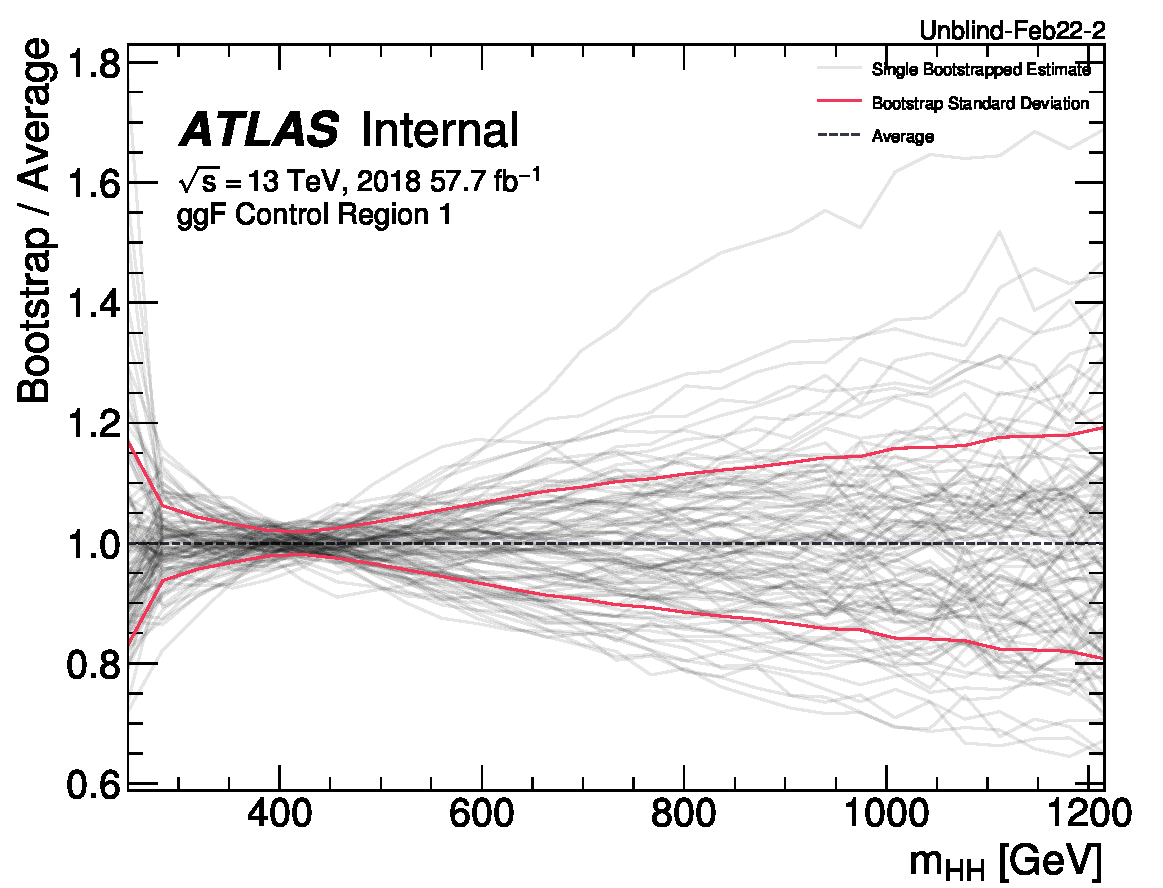
\includegraphics[width=0.48\textwidth]{\figpath/spider-ggF-stdev-Unblind-Feb22-2-m-hh-control-18-4b.pdf}
	}
	\subfloat[]{\label{fig:bootstrap-breakdown-vbf}
		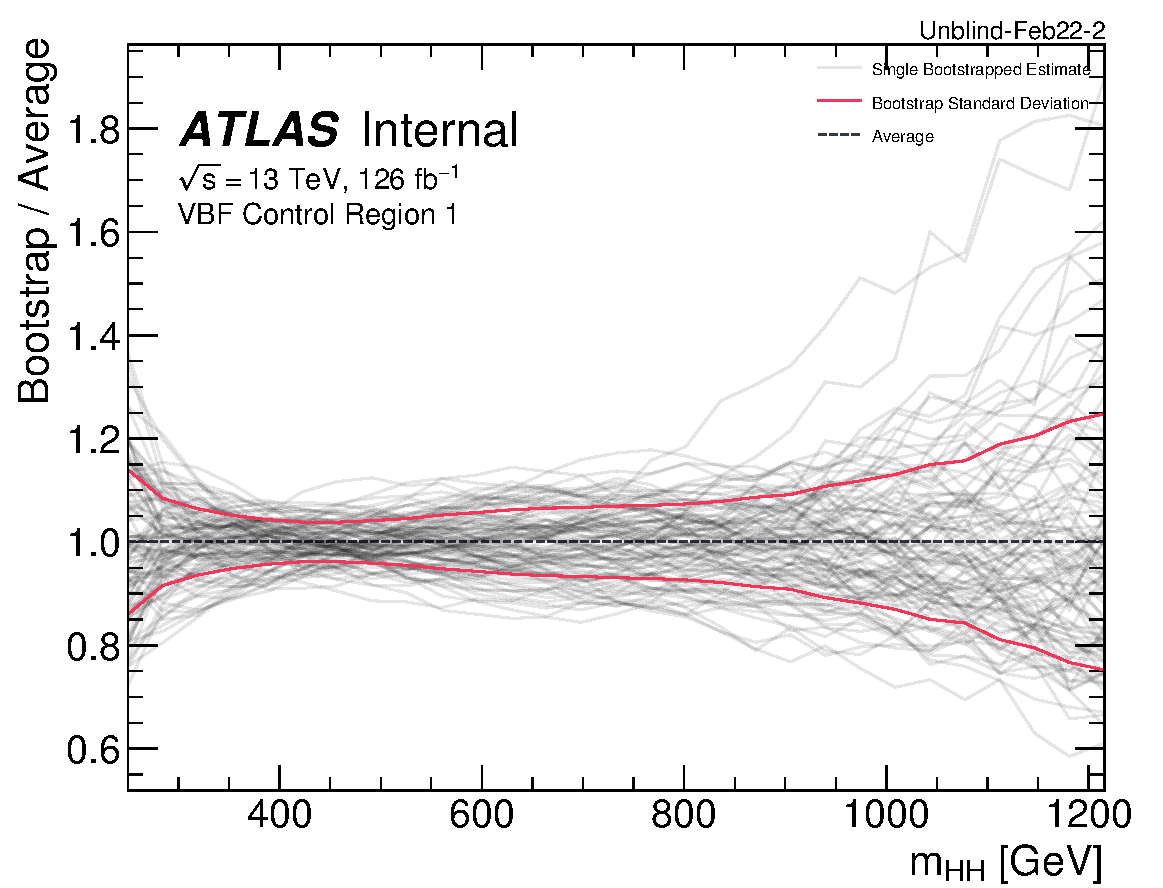
\includegraphics[width=0.48\textwidth]{\figpath/spider-VBF-stdev-Unblind-Feb22-2-m-hh-control-all-4b.pdf}
	}
	\caption{Illustration of the bootstrap band procedure, shown as a ratio to the nominal estimate. 
	Each grey line is from the \mhh prediction for a single bootstrap training, and the solid red line shows the standard deviation of histograms for the 2017 ggF background estimate (left) and VBF years inclusive background estimate (right). 
		}
	\label{fig:bootstrap-breakdown}
\end{figure}

\FloatBarrier
\clearpage

\subsection{Choice of control region}
\label{subsec:shape}

\def\figsversion{V3}
To account for the systematic bias associated with deriving the reweighting function
in CR1, an alternative background
model is derived in CR2.
To aid in deriving an uncertainty to cover this bias, the Signal Region is split into quadrants - four sectors of approximately equal area - where the angle of alignment is set to match the quadrants that define the control regions, CR1 and CR2. The four SR quadrants are named for their relative positions in the Higgs Candidate mass plane, where Q is short for quadrant - Q$_\text{N}$ (north), Q$_\text{S}$ (south), Q$_\text{E}$ (east) and Q$_\text{W}$ (west), and shown in \Fig{\ref{fig:quadNP}}.

\begin{figure}[ht]
    \centering
    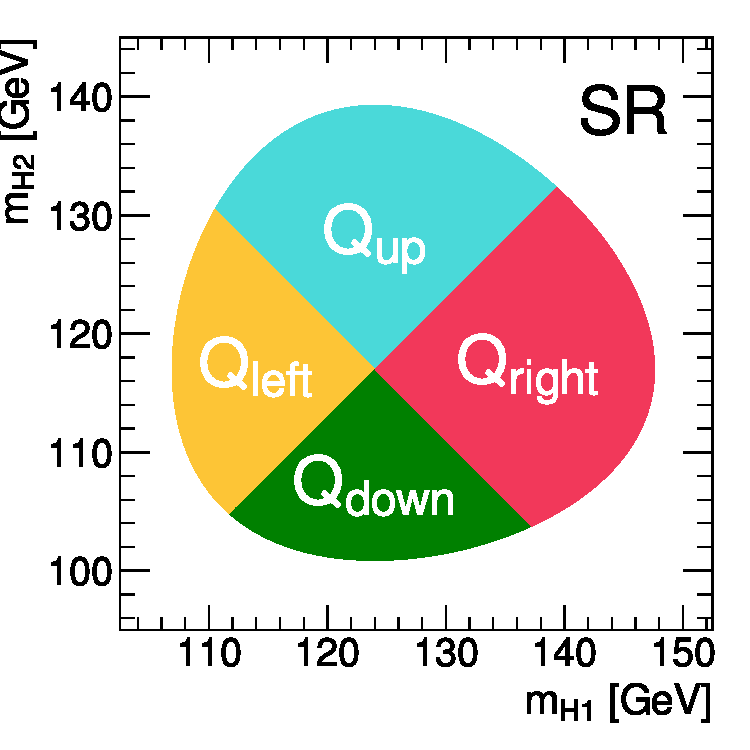
\includegraphics[width=0.48\textwidth]{{figures/nr-int-note/systematics/V3/quadNP_viz.pdf}}		
    \caption{SR quadrants chosen to derive the four background variation nuisance parameters.}
    \label{fig:quadNP}
\end{figure}


The nominal background estimate is derived by applying weights derived in CR1 to all four SR quadrants. Four alternative background estimates are derived by applying weights derived in CR1 to three of the SR quadrants and weights derived in the CR2 to the one remaining SR quadrant. For example, one alternative background estimate is derived by applying CR1-derived weights to Q$_\text{S}$, Q$_\text{E}$ and Q$_\text{W}$, and CR2-derived weights to Q$_\text{N}$. 
The procedure is to reduce the constraints of a single nuisance parameter (NP) if we were to take the whole CR2 weights as a single uncertainty. It constraint was seen in previous 36~\ifb paper and the resonant paper, where certain NP decomposition was also applied.
As we believe the QCD background contains multiple sources, this choice of splitting NPs is to introduce more degrees of freedom to the fit.
This can be done in various ways.
The current way of splitting to four quadrants aligns well with the CR1 and CR2 region definitions, therefore is deemed to be a natural choice.

The difference between the baseline and alternative estimates is used to define a shape uncertainty on the \mhh
spectrum, which is made two-sided by symmetrizing the difference around
the baseline. Note that both normalization and shape differences are taken into considered.

These SR quadrants align with the four sectors of CR1 and CR2 to give these shape systematics the flexibility to naturally follow the kinematic similarity of the adjacent CRs.
The symmetrized difference between the nominal and alternative background estimates are shown for the ggF discriminant for each year in \Figrange{\ref{fig:shapesyst-var-unrolled-16-4b}}{\ref{fig:shapesyst-var-unrolled-18-4b}}. 
Complementary comparisons of the nominal and alternative background estimates for the VBF selection are included in Appendix~\ref{app:vbf_shape_systematics}. 

\def\figsversion{V5}
\def\NNTtag{UNB-MAR21-shuffled}
\def\systID{SR-quads-rot-Xhh-unrolled-syst-m-hh-Signal-Region-NN}
\def\bcat{4b}

%\def\figpath{figures/nr-int-note/systematics/V5/}

\foreach \yr in {16, 17, 18}{
	\begin{figure}[ht]
		\centering
		\subfloat%[Q$_\text{N}$]
		{
			\includegraphics[width=\textwidth]{\figpath\NNTtag-SR-Q1-\systID-\yr-\bcat}
		} \\
		\subfloat%[Q$_\text{S}$]
		{
			\includegraphics[width=\textwidth]{\figpath\NNTtag-SR-Q3-\systID-\yr-\bcat}
		} \\
		\subfloat%[Q$_\text{E}$]
		{
			\includegraphics[width=\textwidth]{\figpath\NNTtag-SR-Q4-\systID-\yr-\bcat}
		} \\		
		\subfloat%[Q$_\text{W}$]
		{
			\includegraphics[width=\textwidth]{\figpath\NNTtag-SR-Q2-\systID-\yr-\bcat}
		}
		\caption{Example of variation in the SR NP quadrants for the 20\yr~ggF~discriminant.}
		\label{fig:shapesyst-var-unrolled-\yr-\bcat}
	\end{figure}
}


\FloatBarrier
\clearpage

\subsection{3b1f non-closure uncertainty}
\label{subsec:syst:3b1fnonclosure}

The 3b1f region is defined such that it contains events with three jets that were b-tagged at the 77\% working point, but that all other jets failed to be b-tagged at even the loosest 85\% working point.
The fourth jet required to reconstruct the di-Higgs is taken as the highest \pt non-b-tagged jet.
The standard methodology for deriving the background estimation (\Sect{\ref{bkg-reweight-method}}) is performed on this region, with 4b events replaced by 3b1f.
The background prediction uncertainties include 2b stat error, bootstrap (\Sect{\ref{sec:subsec:bootstrap}}), and CR1 versus CR2 shape uncertainties (\Sect{\ref{sec:subsec:shape}}).
Detailed studies can be found in \App{\ref{app:3b1f:val}}.
A small deviation between the reweighted 2b and the 3b1f data distributions in the SR was found in the ggF channel but not in the VBF channel.
An additional uncertainty due to the 3b1f non-closure is derived for the ggF channel to cover this deviation.

The uncertainty is derived as follows:
In each of the analysis categories (\Sect{\ref{subsec:cat-motivation}}), the ratio of the 3b1f and the reweighted 2b \mhh distributions is computed using the binning described in \Tab{\ref{tab:binning-hyperparameters}}.
The ratio is compared to unity bin by bin.
If the difference is not covered by the quadratic sum of the background prediction uncertainties and the 3b1f data statistical uncertainty in that bin, the residual is taken to form a template.
To reduce the statistical fluctuations between bins, the template is smoothed by averaging each bin with its two neighboring bins.
The smoothed template is used as a non-closure uncertainty in 4b.

\FloatBarrier
\clearpage
\subsubsection{Summary of Background Modeling Uncertainties}
\label{subsec:bkgUnc-summary}

\def\NNTtag{NR-MAR22-unblind}

Relative magnitudes of the uncertainties for
each year are shown in \Tab{\ref{tbl:ggF-errs-ALL}} for ggF and \Tab{\ref{tbl:VBF-errs-ALL}} for VBF along with an estimate of the impact of the statistics of 4b
data in the signal region on the total error. 

\input{tables/\NNTtag-VBF-error-table-ALL.tex}
\input{tables/\NNTtag-ggF-error-table-ALL.tex}

A visualization of the magnitudes of these templates for the ggF channels is shown in \Fig{\ref{fig:bkgRelErr-ggF-4b}} and VBF in \Fig{ref{fig:bkgRelErr-VBF-4b}}.
The statistical error dominates for high \mhh while the shape systematic from the difference in the CR1 and CR2 contributes more in the moderate \mhh region that drives our analysis sensitivity.
Although the stat error (from the limited 2b data statistics) is negligible relative to the bootstrap error in the bulk of the distribution, it becomes relevant in the high \mhh tail. 
The final statistical uncertainty used for the limit setting is therefore the sum (in quadrature) of these two components. 

\def\NNTtag{NR-UNBLIND-FEB22-2}

\begin{figure}[ht]
	\centering
	\subfloat[\bcat \ 2016 ggF]{
		\includegraphics[width=\textwidth]{\figpath\NNTtag-ggF-relError-16-4b}
	} \\
	\subfloat[\bcat \ 2017 ggF]{
			\includegraphics[width=\textwidth]{\figpath\NNTtag-ggF-relError-17-4b}
	} \\
	\subfloat[\bcat \ 2018 ggF]{
			\includegraphics[width=\textwidth]{\figpath\NNTtag-ggF-relError-18-4b}
	}
	\caption{Relative error contributions of the background for the \bcat~ggF~discriminant.}
	\label{fig:bkgRelErr-ggF-4b}
\end{figure}


\begin{figure}[ht]
	\centering
		\includegraphics[width=0.45\textwidth]{\figpath\NNTtag-VBF-relError-all-4b-dEta_1.pdf}
		\includegraphics[width=0.45\textwidth]{\figpath\NNTtag-VBF-relError-all-4b-dEta_2.pdf}
	\caption{Relative error contributions of the background for the \bcat~VBF~discriminant.}
	\label{fig:bkgRelErr-VBF-4b}
\end{figure}

\subsection{Choice of background systematic parametrization}
\label{subsec:bkgUnc-stats}

OK - I made these plots... I just need to \emph{pop} them in from somewhere else!

% I'm not sure if I wrote this or not - I don't think I did tbh
%The signal extraction fit is performed in the \mhh variable, due to its separation power between signal and background, but also between different signal hypotheses (such as different $\kappa_\lambda$ signals). 
%The fit is performed with binned histograms, with the binning defined in \Sect{\ref{subsec:cat-motivation}}, in different categories, defined in \Sect{\ref{subsubsec:ggF-cats}} for the ggF selection and in \Sect{\ref{subsubsec:VBF-cats}} for VBF. 
%
%\textbf{For the ggF channel, the fit is performed for each one of the three data taking years separately.} This choice is informed by the background estimate strategy, where the neural network is trained, and shape uncertainties are assessed, separately per year. This choice leads to lower background estimate uncertainties with respect to an all-years together training, with a similar nominal estimate between both options. This is due to large difference in kinematics between the years cause by different trigger thresholds (on both jet $p_T$ and online \Pqb-tagging). On the other hand, \textbf{the years are treated inclusively for the VBF channel}, both on the background estimate step and on the fitting step. The main performance bottleneck for the VBF selection background estimate is the available statistics to train the neural network. In this case, statistics are more important than the different kinematics between the years. Therefore, obtaining the background inclusively in years is preferred.

%\subsection{Background Shape Nuisance Parameter Correlation Scheme}
%\label{subsec:stats-corr-scheme}

The number of categories, fits and all possible background nuisance parameters are described in table \ref{stat:fit-table}, informed by the fitting strategy described in the previous sub-section.  
For both VBF and ggF channels, the shape and normalization uncertainties for each category are obtained separately by comparing the CR1 and CR2 models after each category selection.

\begin{table}[!htbp]
    \centering
    \begin{tabular}{c|c|c}
{} & ggF channel & VBF channel \\ \hline
Categories & \begin{tabular}[c]{@{}c@{}}3 years\\ $\times$ 3 $|\Delta\eta_{HH}|$ \\ $\times$ 2 $X_{HH}$ \\ = 18 categories\end{tabular} & 2 $|\Delta\eta_{HH}|$ categories \\ \hline
\begin{tabular}[c]{@{}c@{}}Background shape\\nuisance parameters\end{tabular} & \begin{tabular}[c]{@{}c@{}}3 years \\  $\times$ $(Q_{\text{N}}, Q_{\text{E}}, Q_{\text{S}}, Q_{\text{W}})$ \\  = 12 \end{tabular} & \begin{tabular}[c]{@{}c@{}} $(Q_{\text{N}}, Q_{\text{E}}, Q_{\text{S}}, Q_{\text{W}})$ \\  = 4\end{tabular} \\ \hline
\begin{tabular}[c]{@{}c@{}}3b1f non-closure\\nuisance parameters\end{tabular} & 18 (1 per category) & 0 \\
\end{tabular}
    \caption{Summary of categorization strategy and background-related nuisance parameters in ggF and VBF analyses.}
\label{stat:fit-table}
\end{table}

These nuisance parameters are not necessarily completely uncorrelated, and a choice on the correlation scheme must be made to perform the fit. 
The main argument for correlating the background shape nuisance parameters across kinematic regions is due to the neural network reweighting. 
The reweighting is trained inclusively with respect to kinematic categories, per year (for the ggF channel) or for all years together (for VBF). 
Possible mismodelings occuring due to the neural network's performance, or, more importantly, its ability to interpolate into the signal region, will therefore have the same source. 
For the VBF channel, one step ahead is taken, and the fit is performed inclusively for all the years for this reason. 
This approach, however, was observed to be detrimental to the ggF background modeling performance, due to the kinematic differences between the years, and is not done. 

Another important indication that these nuisance parameters should be correlated across kinematic regions is the relative impact they have in the \mhh fitting variable. 
This can be seen on Figure \ref{fig:sr-np-impact}, which shows the nuisance parameter relative variations within each quadrant and each year of the ggF analysis. 
Most variations have very similar impacts on \mhh , which corroborates the hypothesis of correlated variations. 

\def\figpath{figures/nr-int-note/unblind_results/V5/}
\begin{figure}[ht]
	\centering
	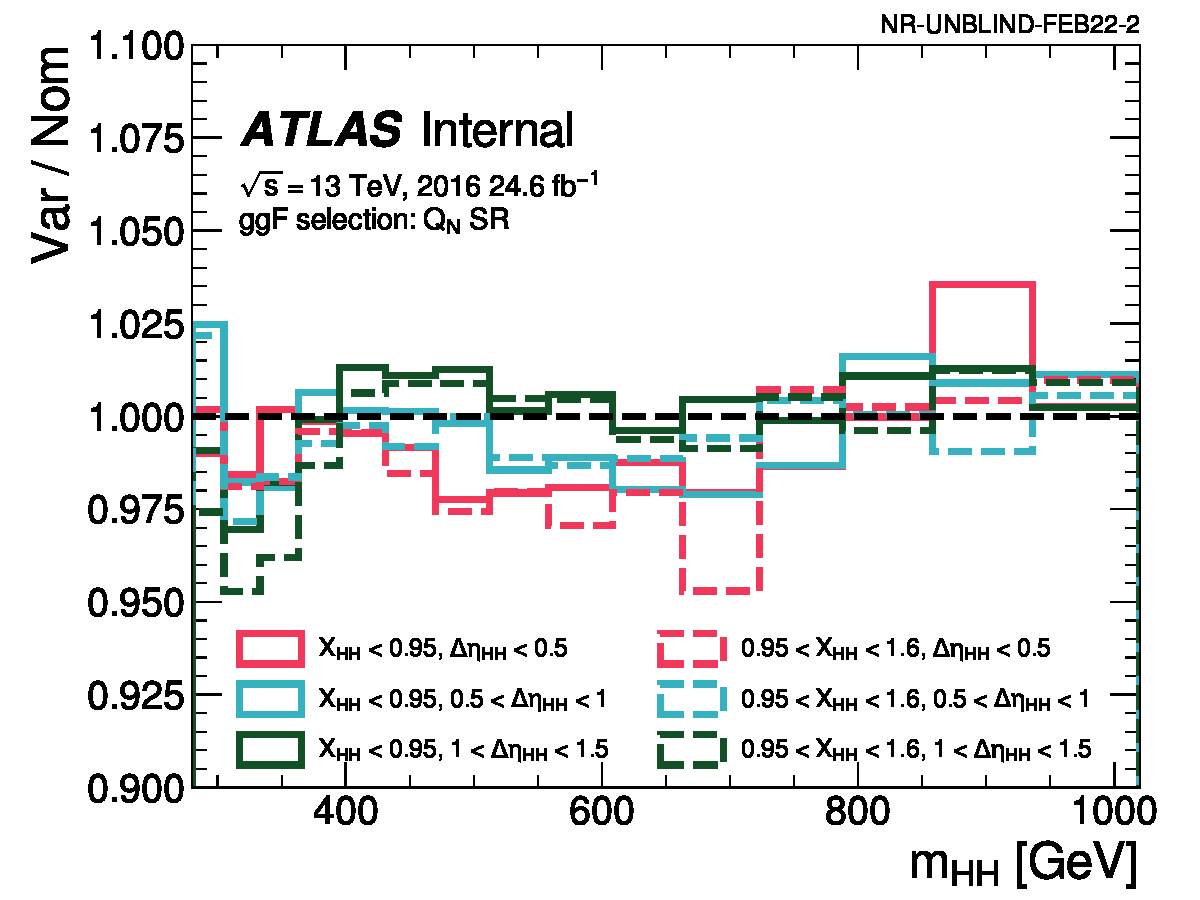
\includegraphics[width=0.32\textwidth]{\figpath/SR_Q1_16}
	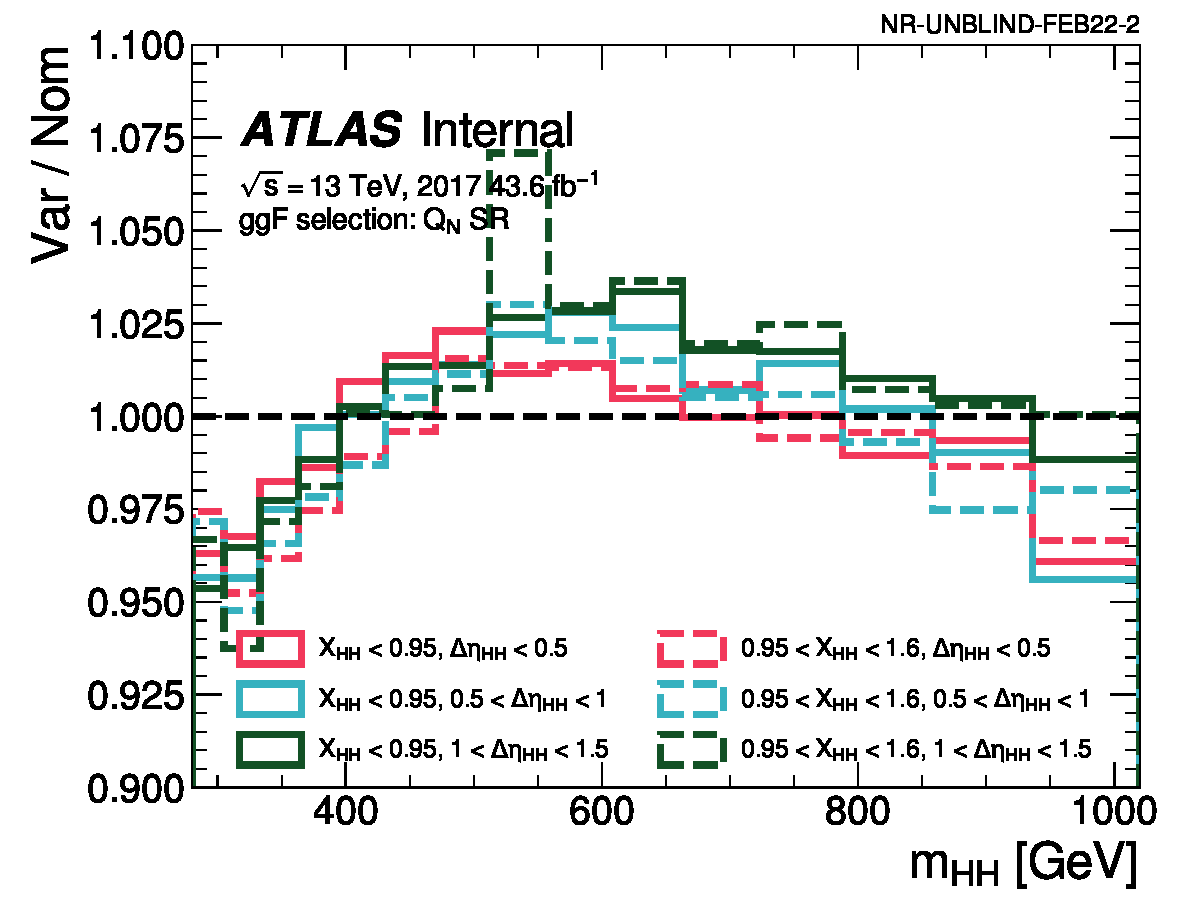
\includegraphics[width=0.32\textwidth]{\figpath/SR_Q1_17}
	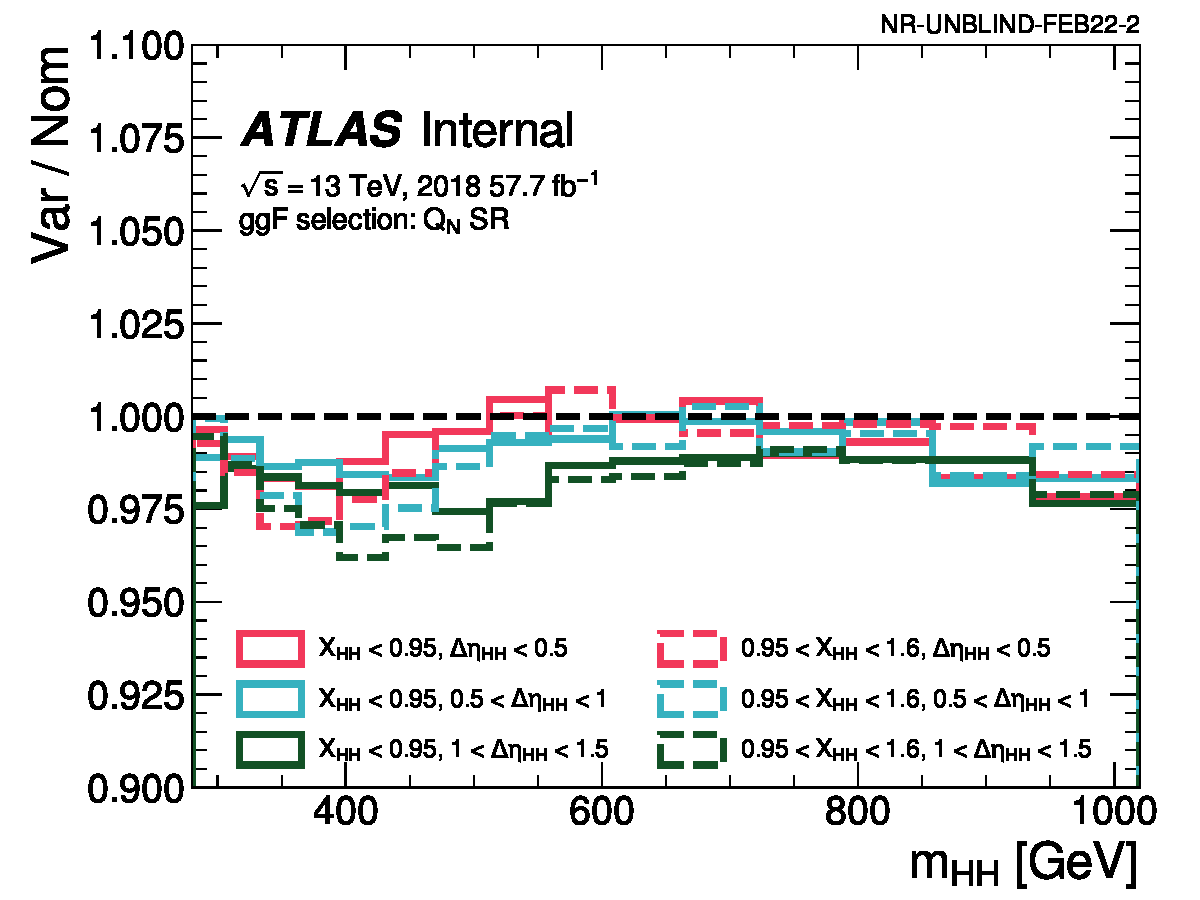
\includegraphics[width=0.32\textwidth]{\figpath/SR_Q1_18}
	\\
	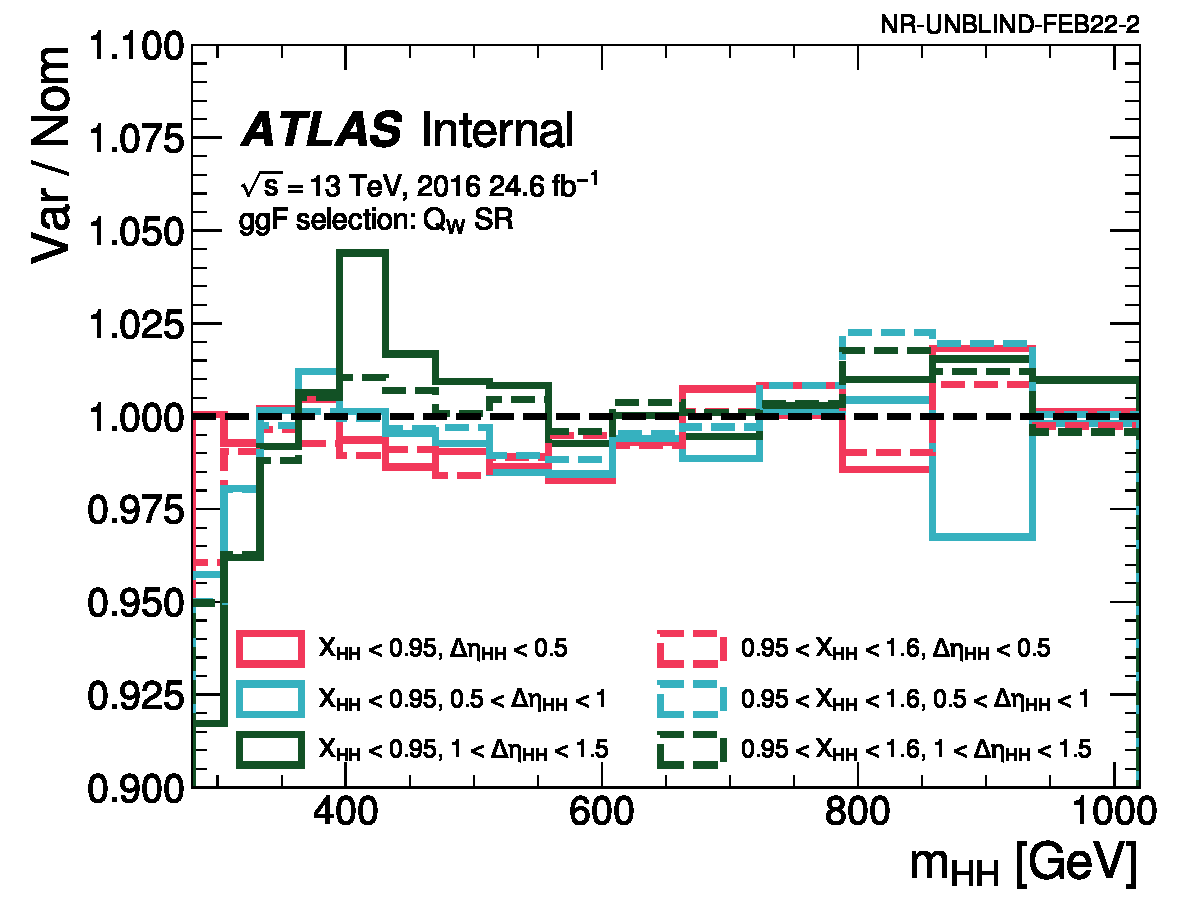
\includegraphics[width=0.32\textwidth]{\figpath/SR_Q2_16}
	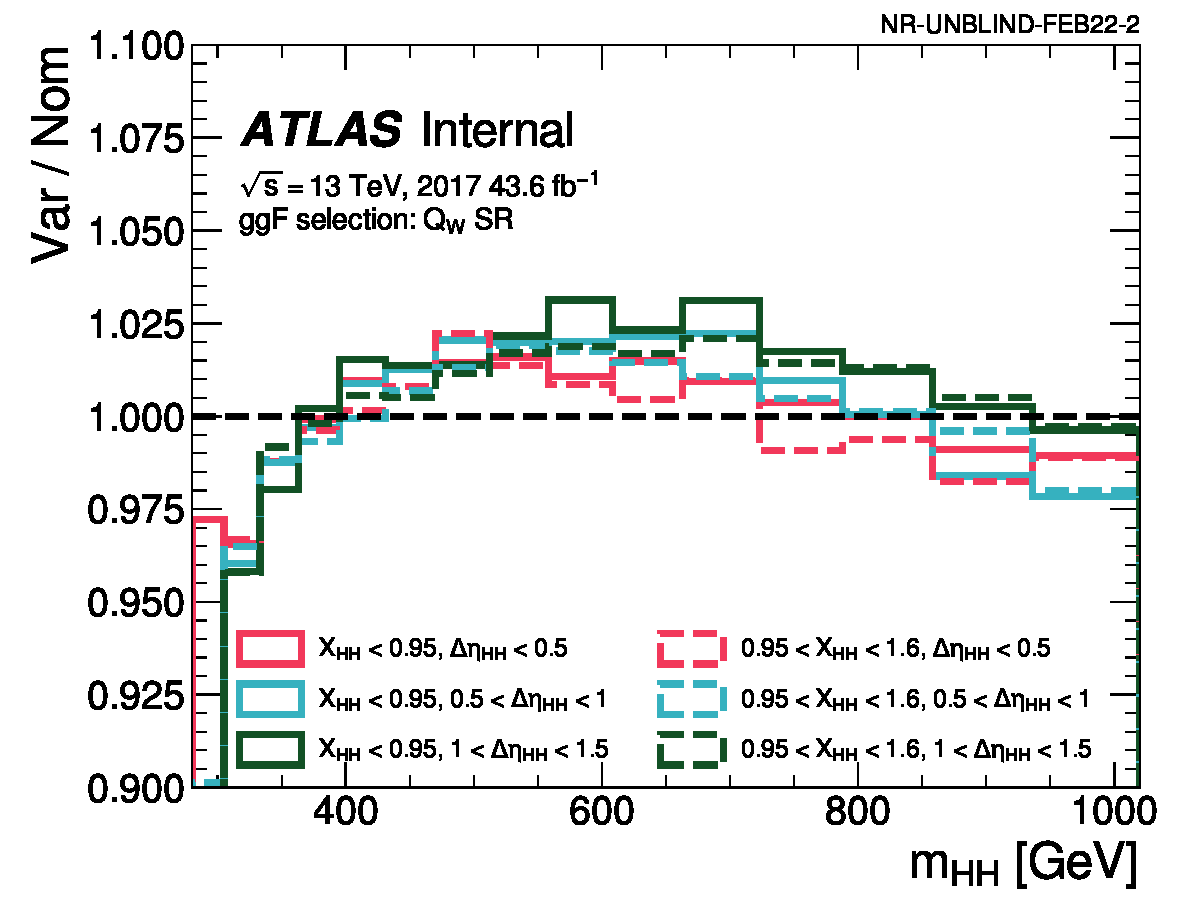
\includegraphics[width=0.32\textwidth]{\figpath/SR_Q2_17}
	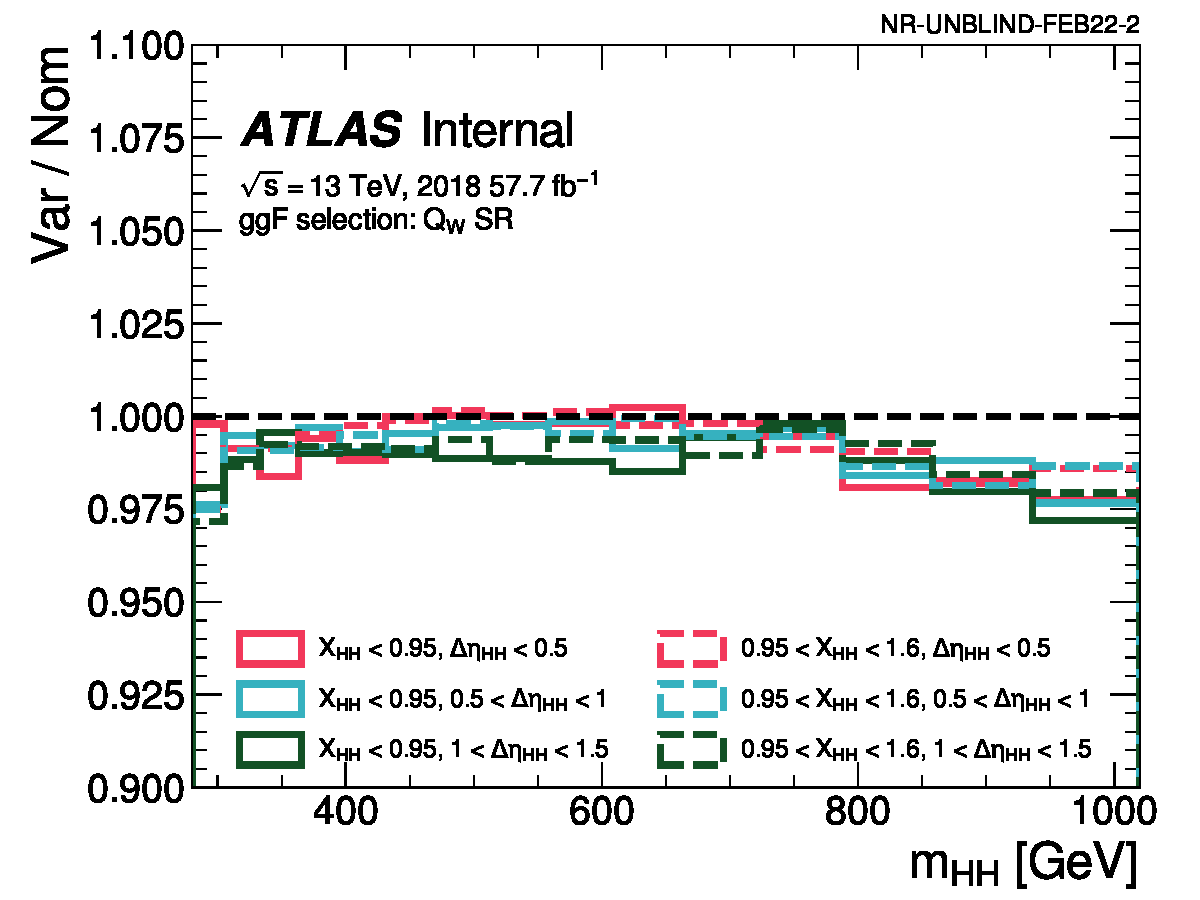
\includegraphics[width=0.32\textwidth]{\figpath/SR_Q2_18}
	\\
	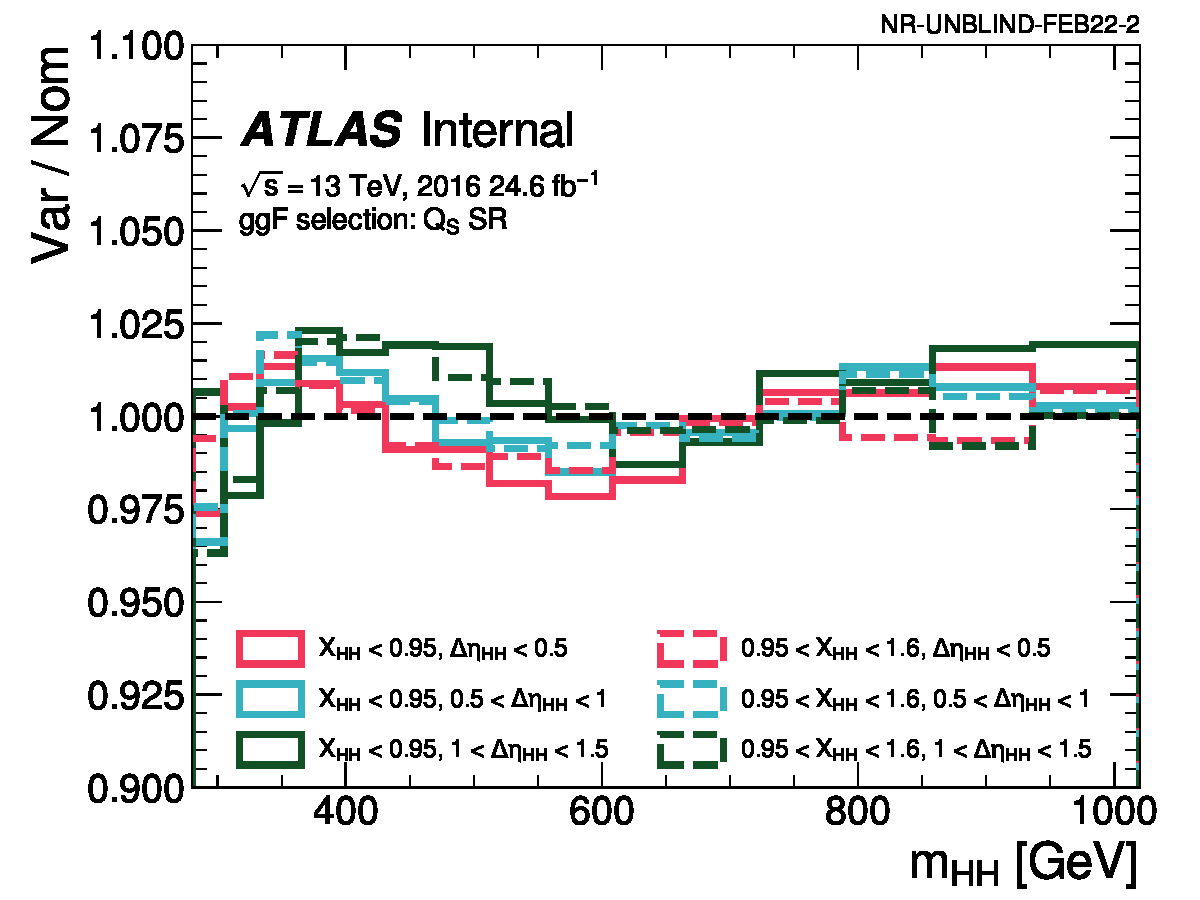
\includegraphics[width=0.32\textwidth]{\figpath/SR_Q3_16}
	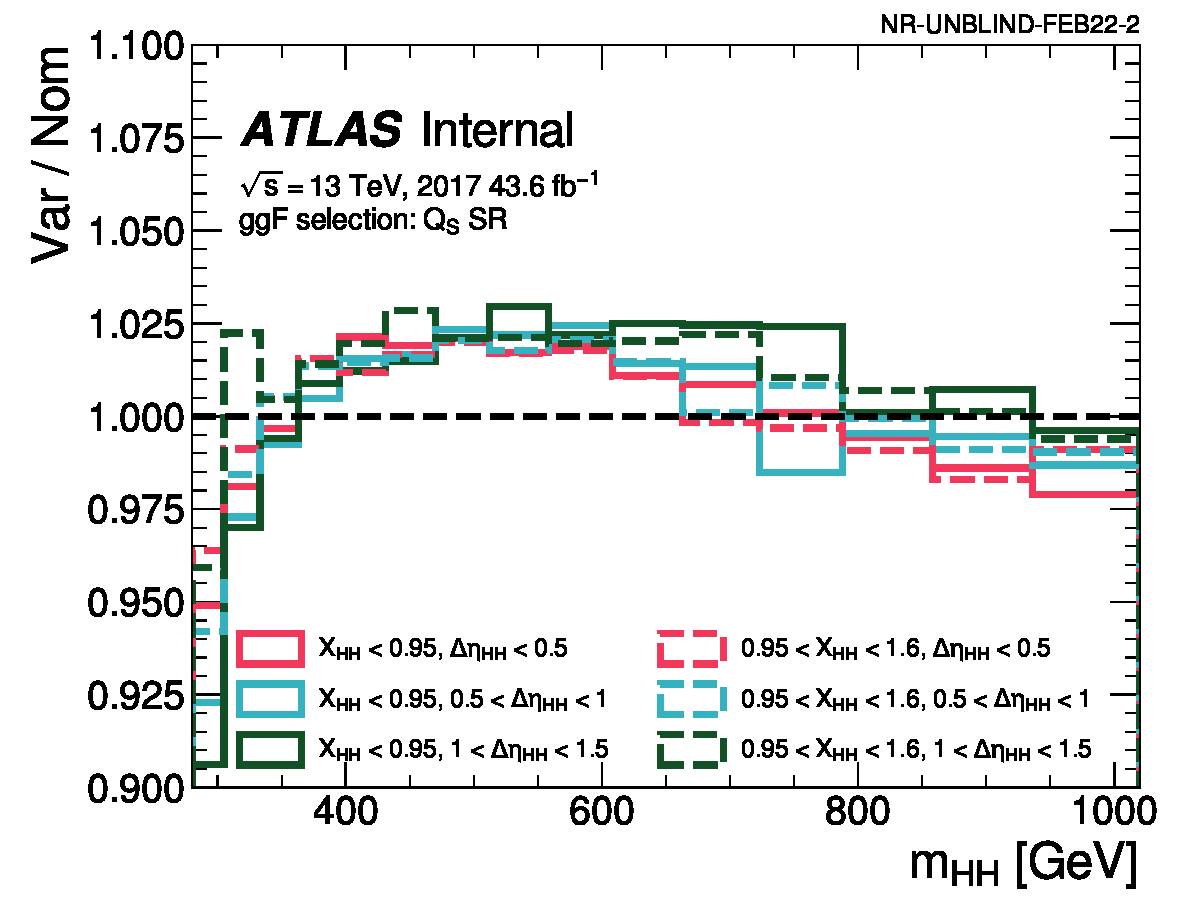
\includegraphics[width=0.32\textwidth]{\figpath/SR_Q3_17}
	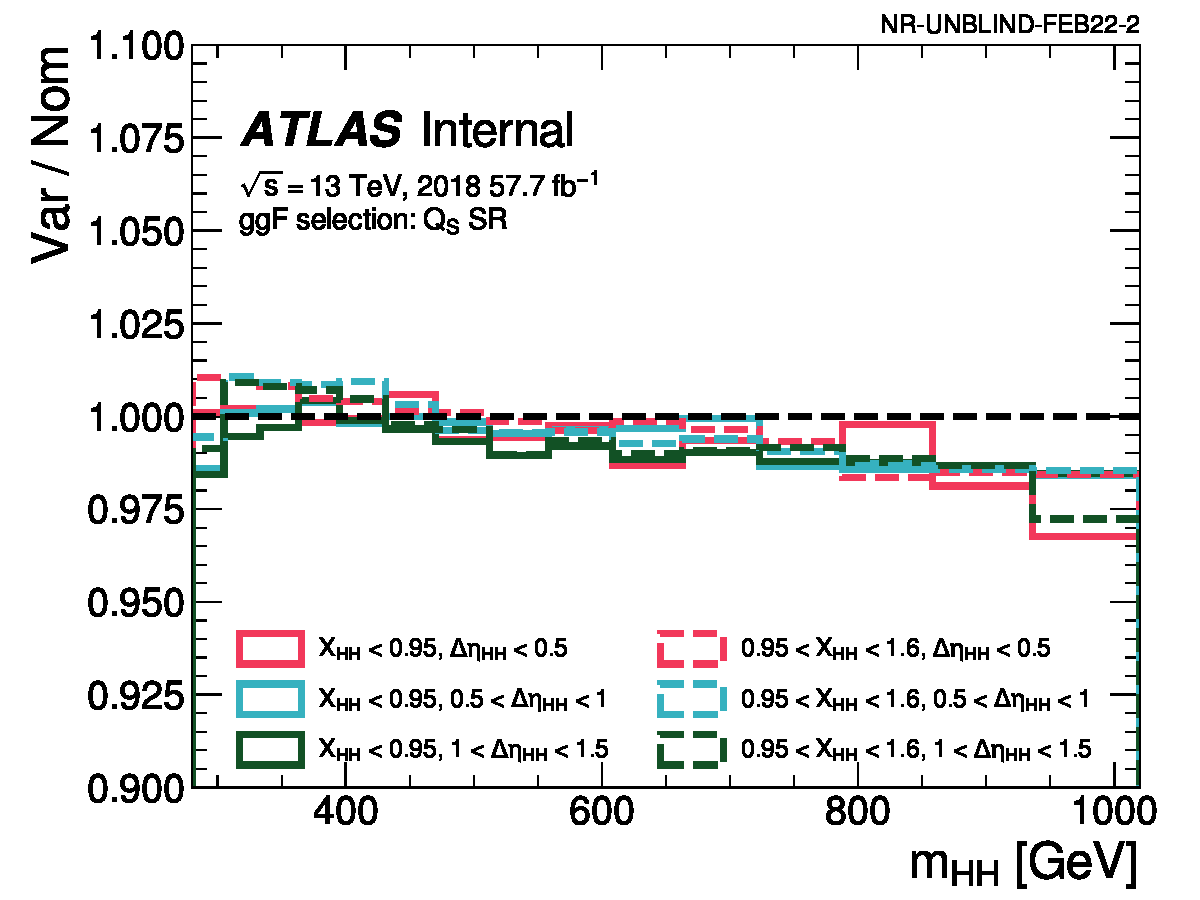
\includegraphics[width=0.32\textwidth]{\figpath/SR_Q3_18}
	\\
	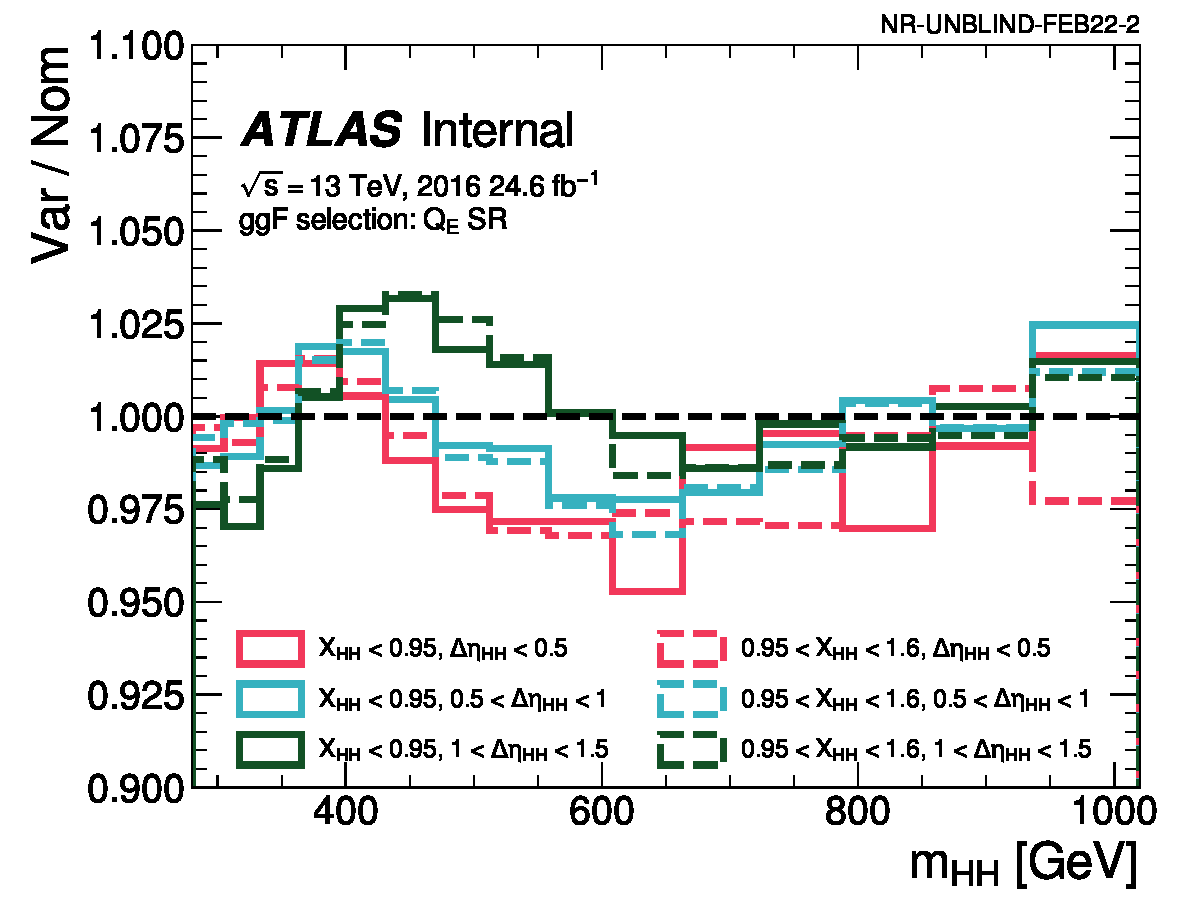
\includegraphics[width=0.32\textwidth]{\figpath/SR_Q4_16}
	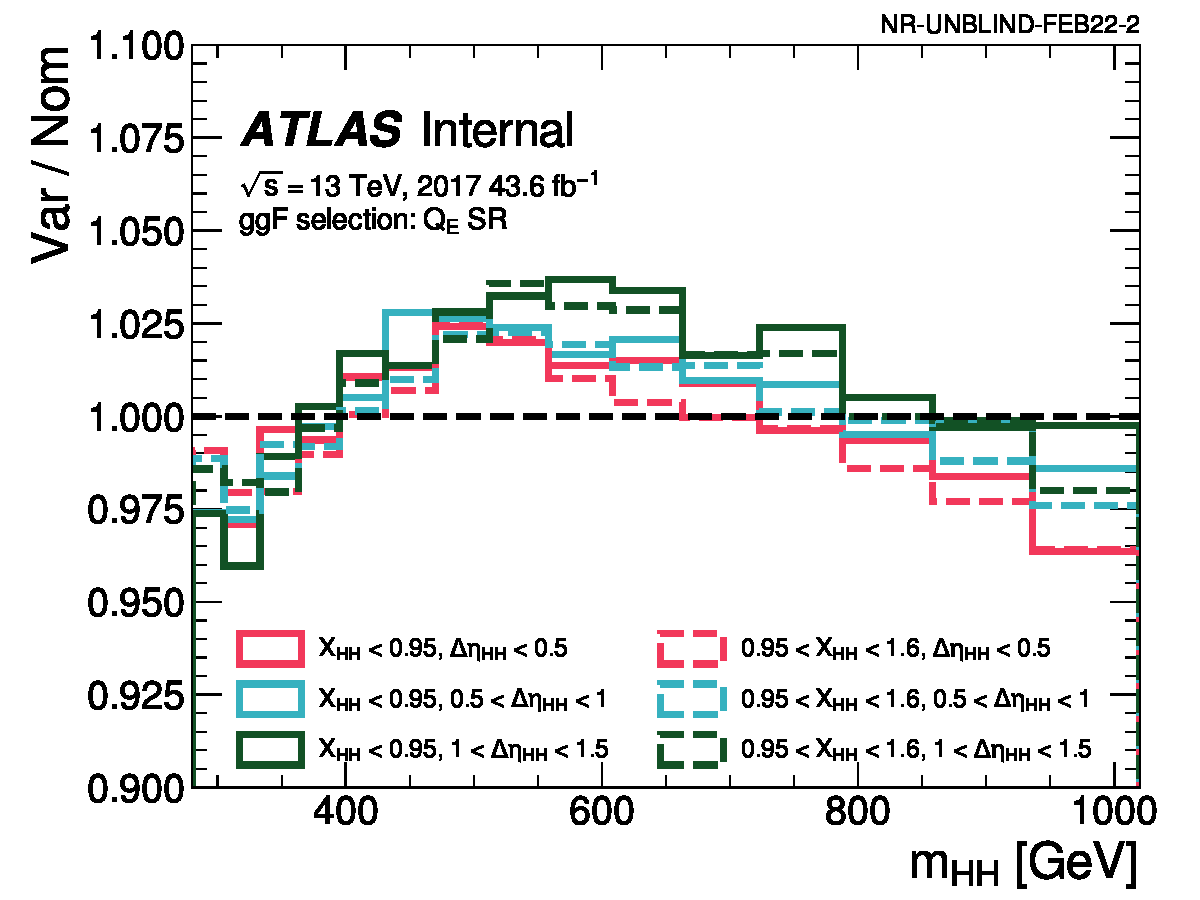
\includegraphics[width=0.32\textwidth]{\figpath/SR_Q4_17}
	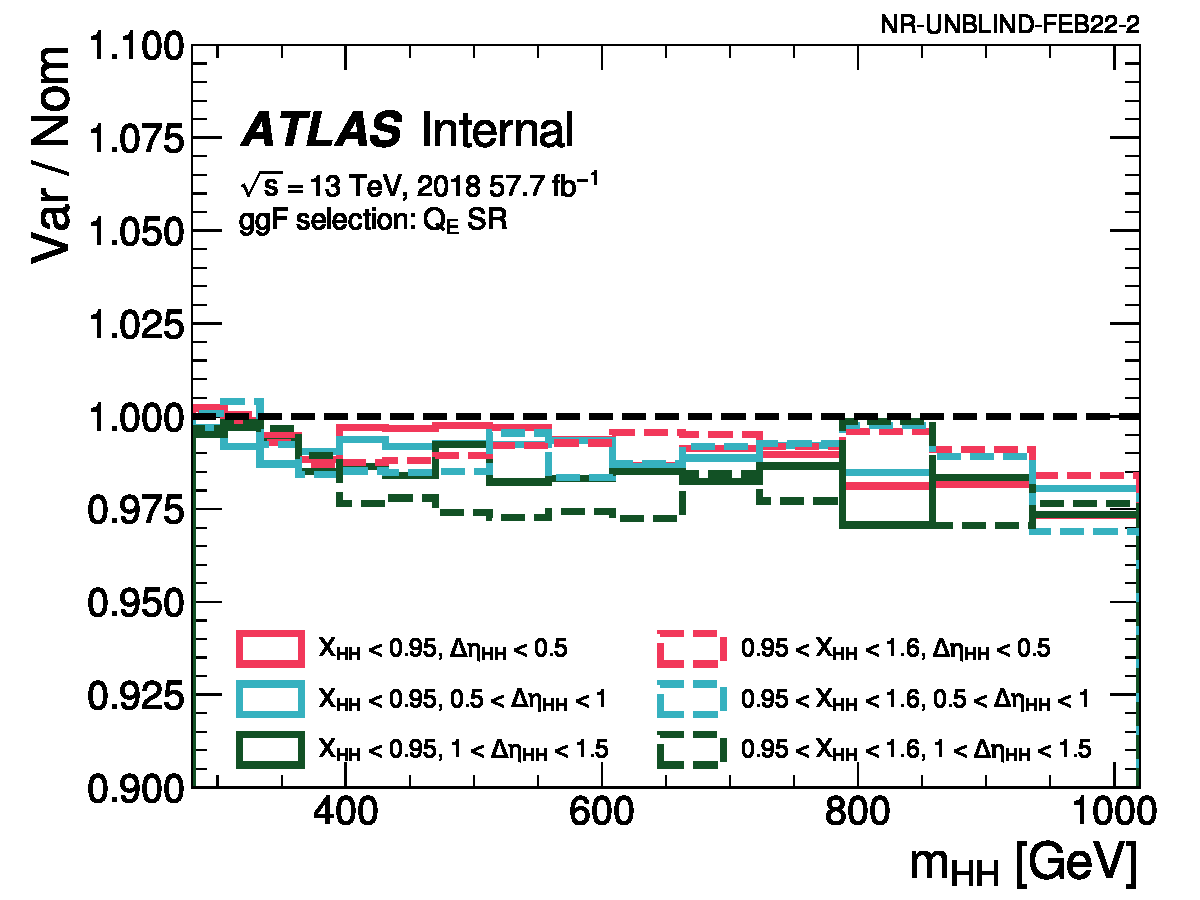
\includegraphics[width=0.32\textwidth]{\figpath/SR_Q4_18}
	\caption{Impact of background shape nuisance parameter variation on \mhh in different kinematic categories for the ggF channel. Each column is a different year for the ggF channel templates while the rows show the SR NP quadrants.}	 
	\label{fig:sr-np-impact}
\end{figure}

\FloatBarrier

Given the arguments above, we choose to correlate the background shape nuisance parameters across kinematic categories, within a year and each quadrant. 
Therefore, the number of free nuisance parameters in the ggF fit related to the background shape is reduced from 72 (3 years $\times$ 6 categories $\times$ $ (Q_{\text{N}}, Q_{\text{E}}, Q_{\text{S}}, Q_{\text{W}})$)  to 12 (3 years $\times (Q_{\text{N}}, Q_{\text{E}}, Q_{\text{S}}, Q_{\text{W}})$). 

For completeness, we also show the templates by category with the different quadrant contributions overlaid in \Fig{\ref{fig:sr-np-impact-by-cat}}.

\begin{figure}[ht]
	\centering
	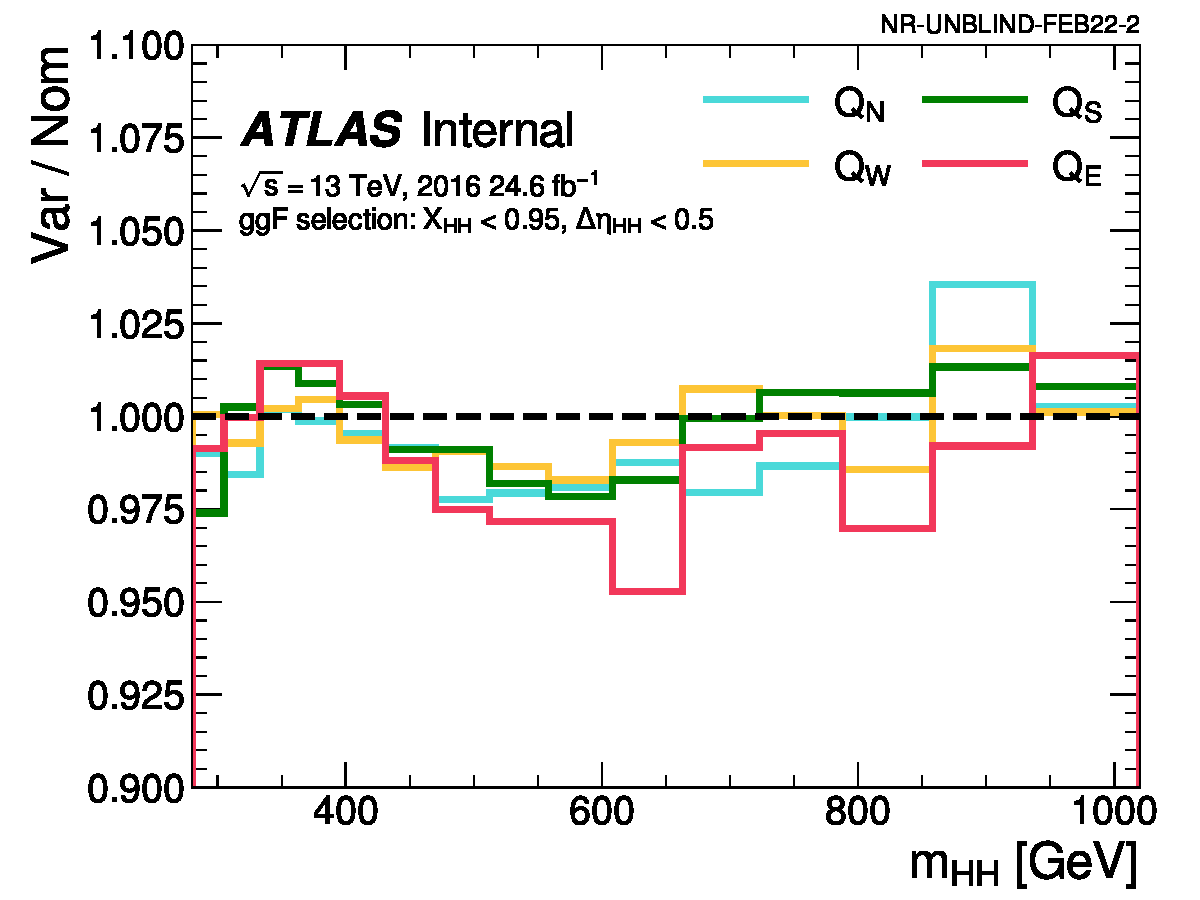
\includegraphics[width=0.3\textwidth]{\figpath/dEta_1_Xhh_1_16}
	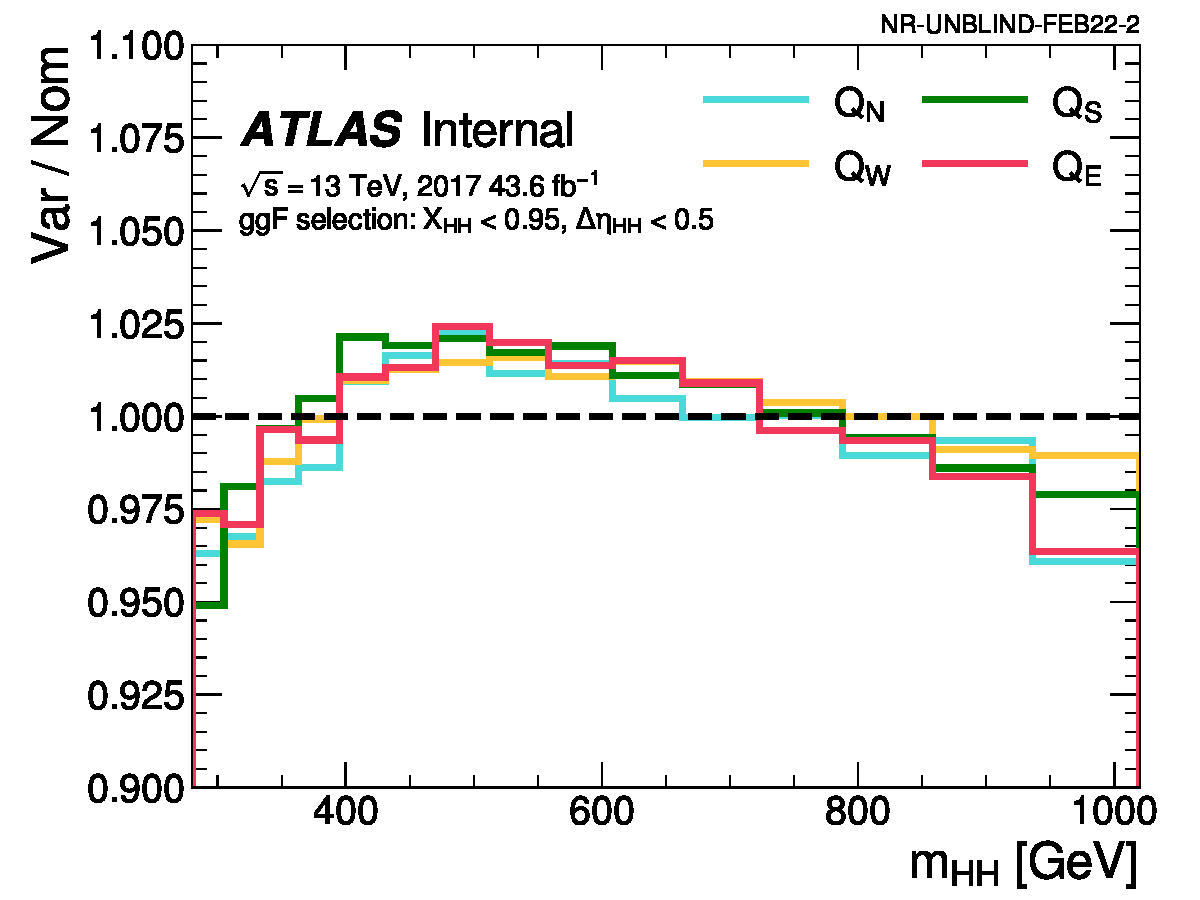
\includegraphics[width=0.3\textwidth]{\figpath/dEta_1_Xhh_1_17}
	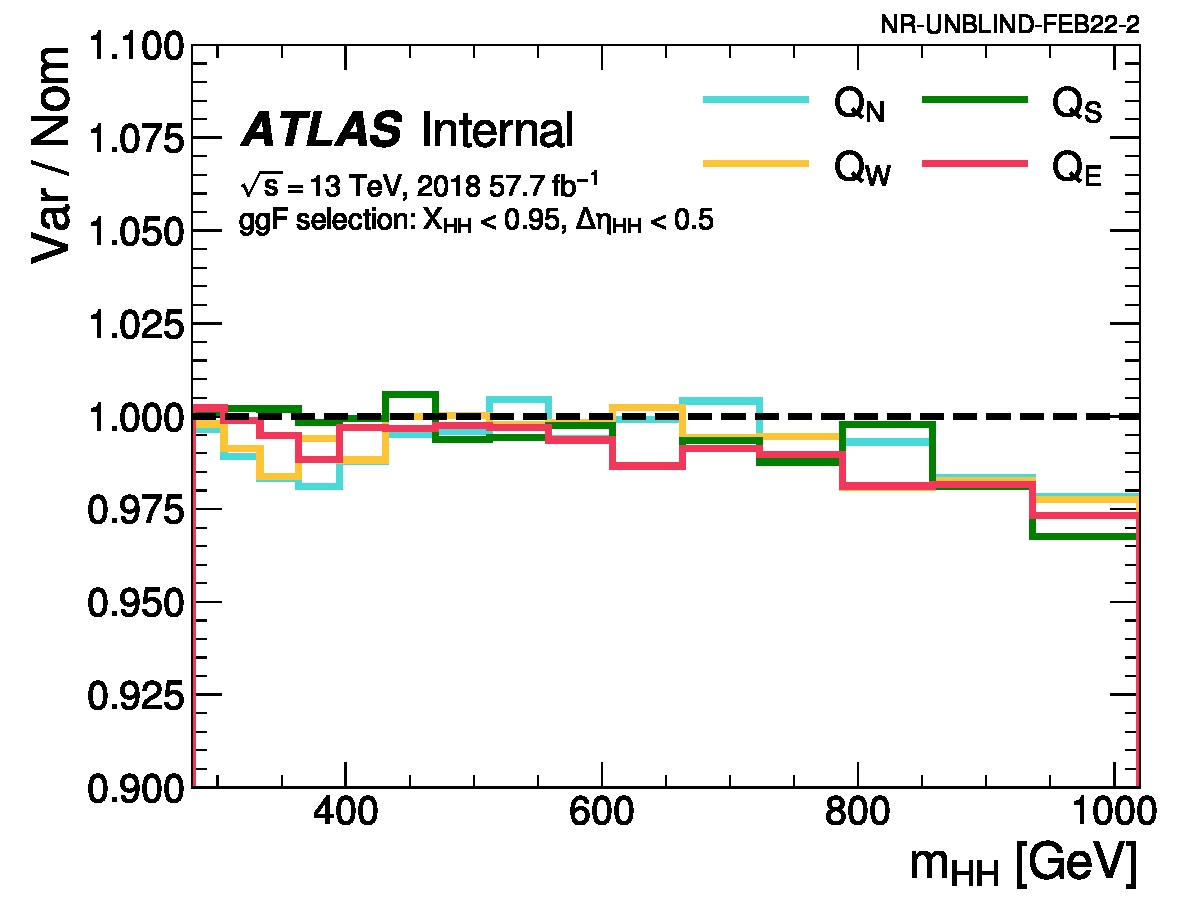
\includegraphics[width=0.3\textwidth]{\figpath/dEta_1_Xhh_1_18}
	\\
	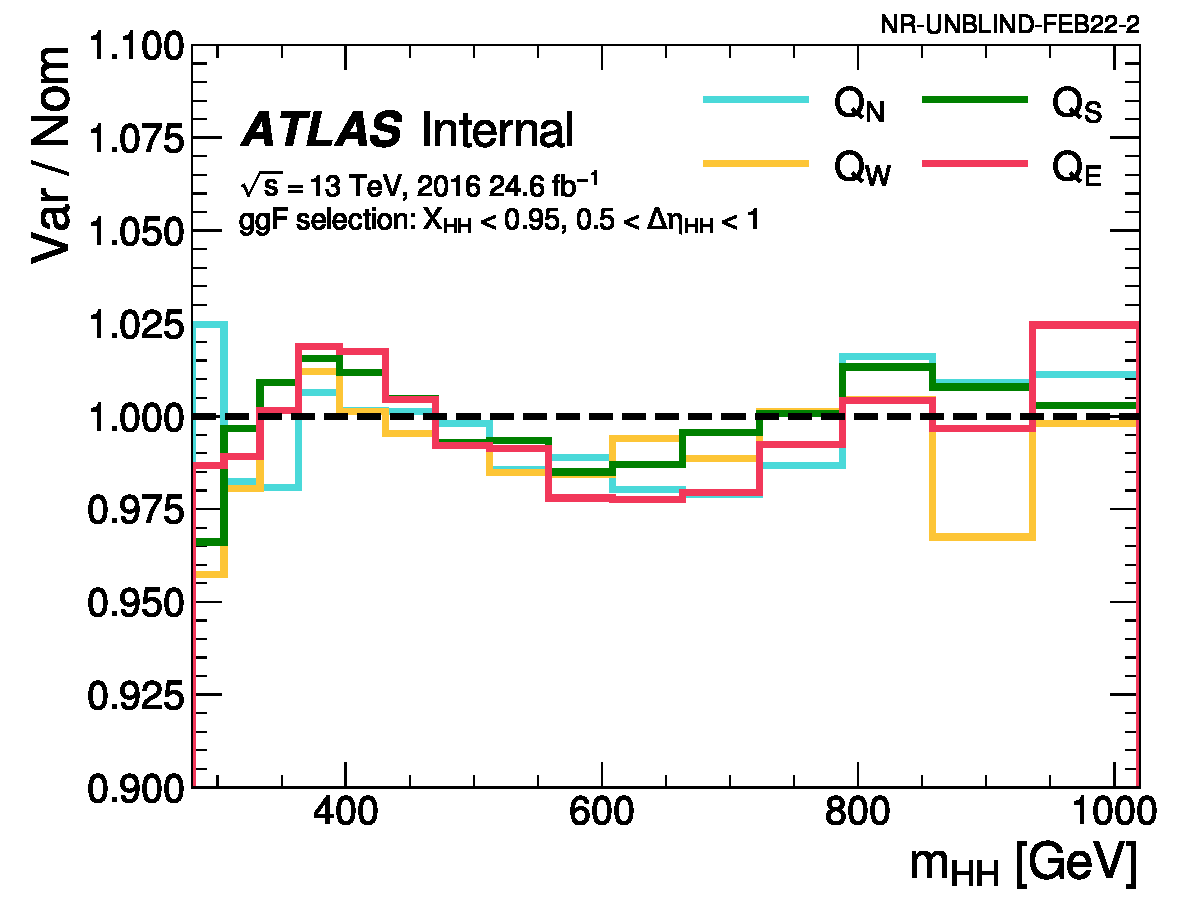
\includegraphics[width=0.3\textwidth]{\figpath/dEta_2_Xhh_1_16}
	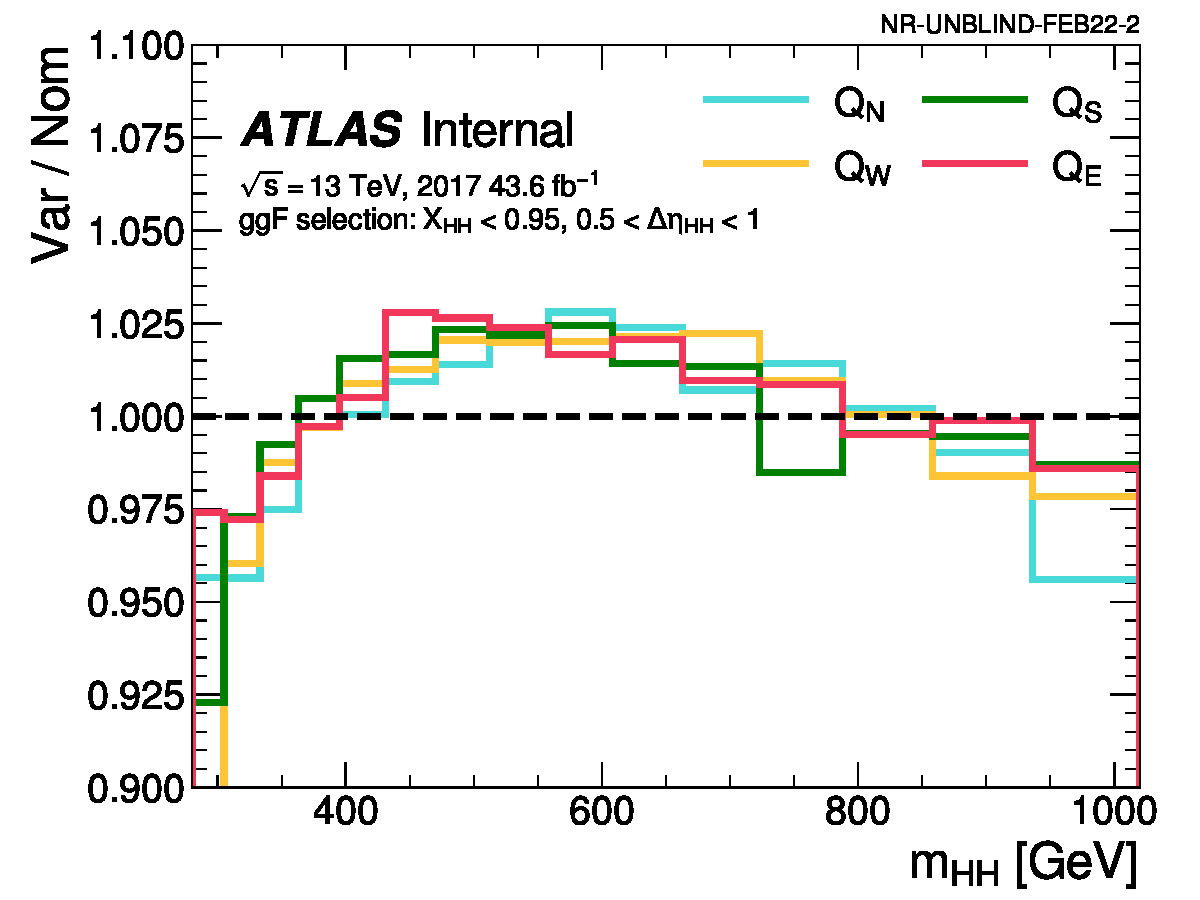
\includegraphics[width=0.3\textwidth]{\figpath/dEta_2_Xhh_1_17}
	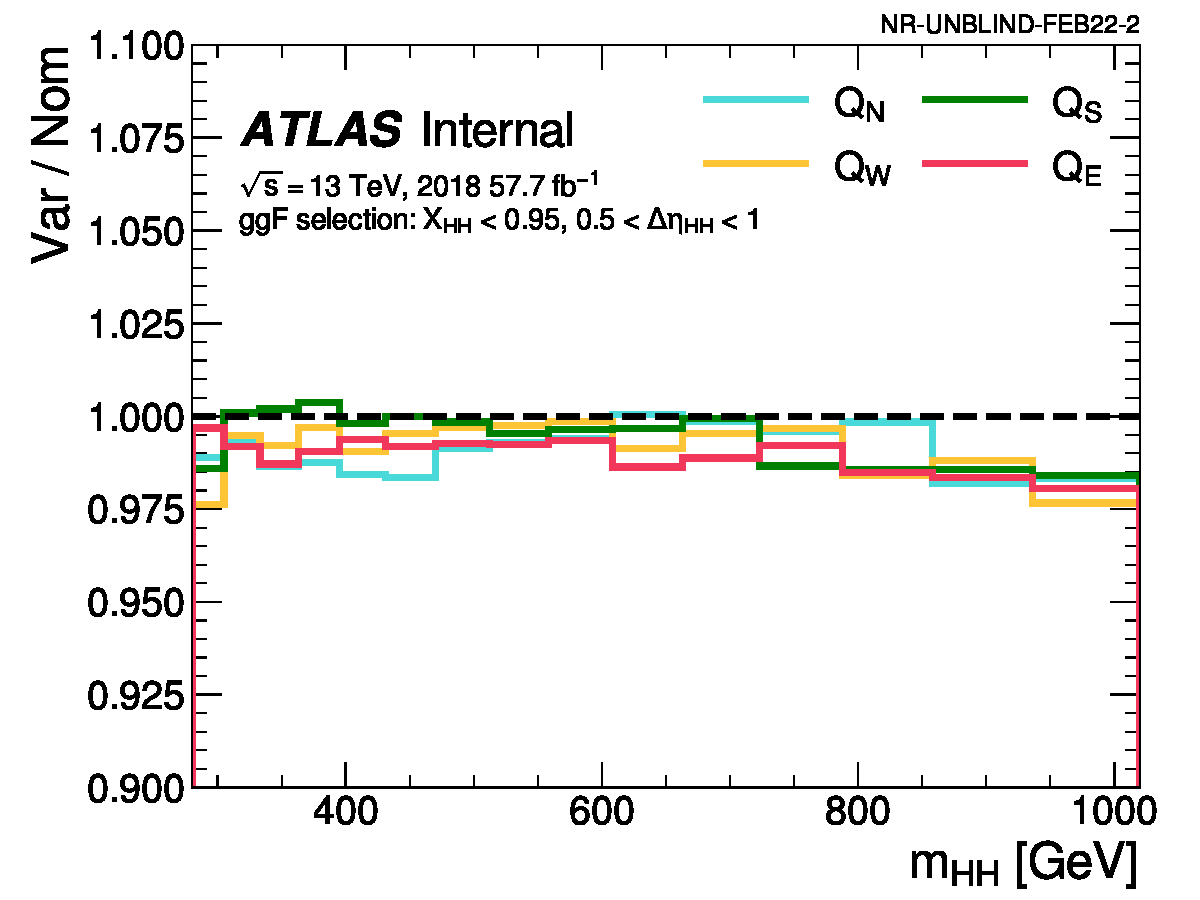
\includegraphics[width=0.3\textwidth]{\figpath/dEta_2_Xhh_1_18}
	\\
	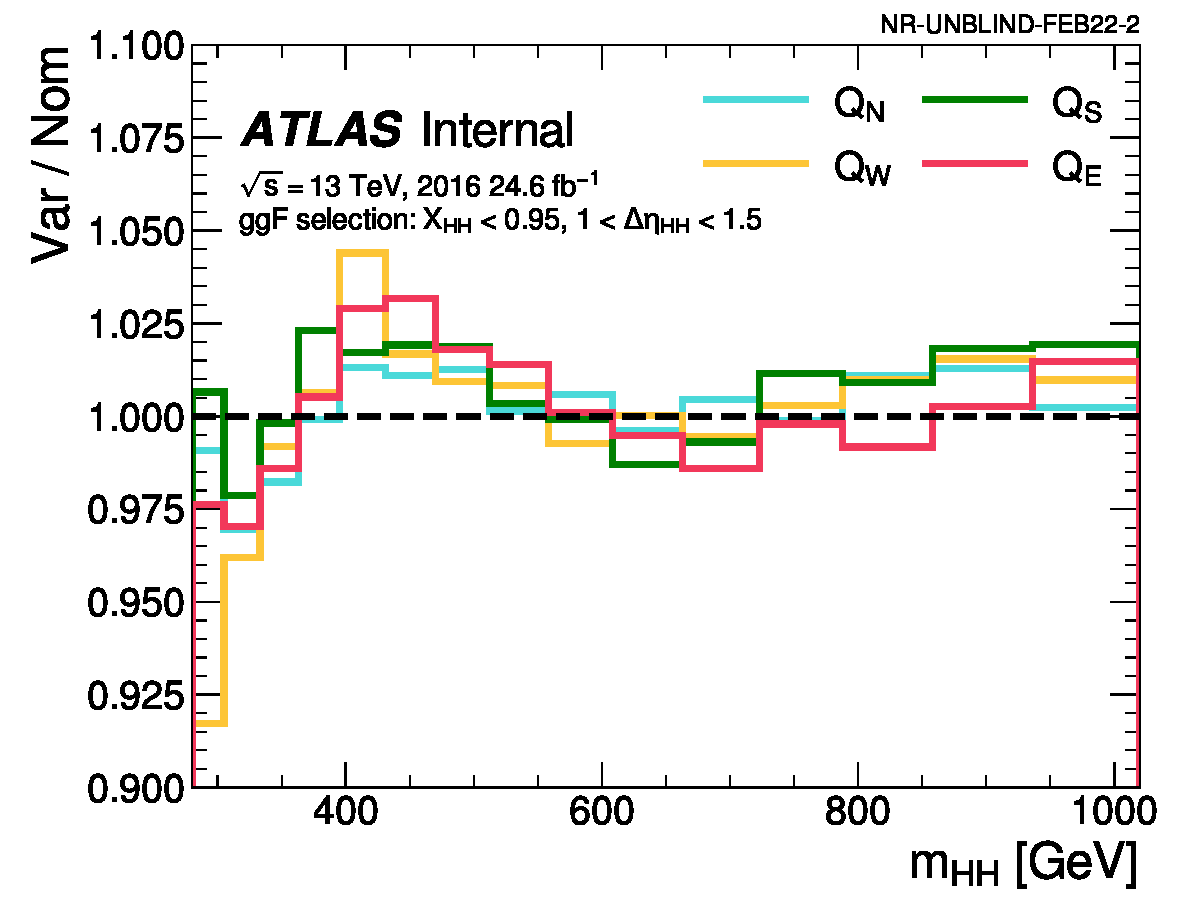
\includegraphics[width=0.3\textwidth]{\figpath/dEta_3_Xhh_1_16}
	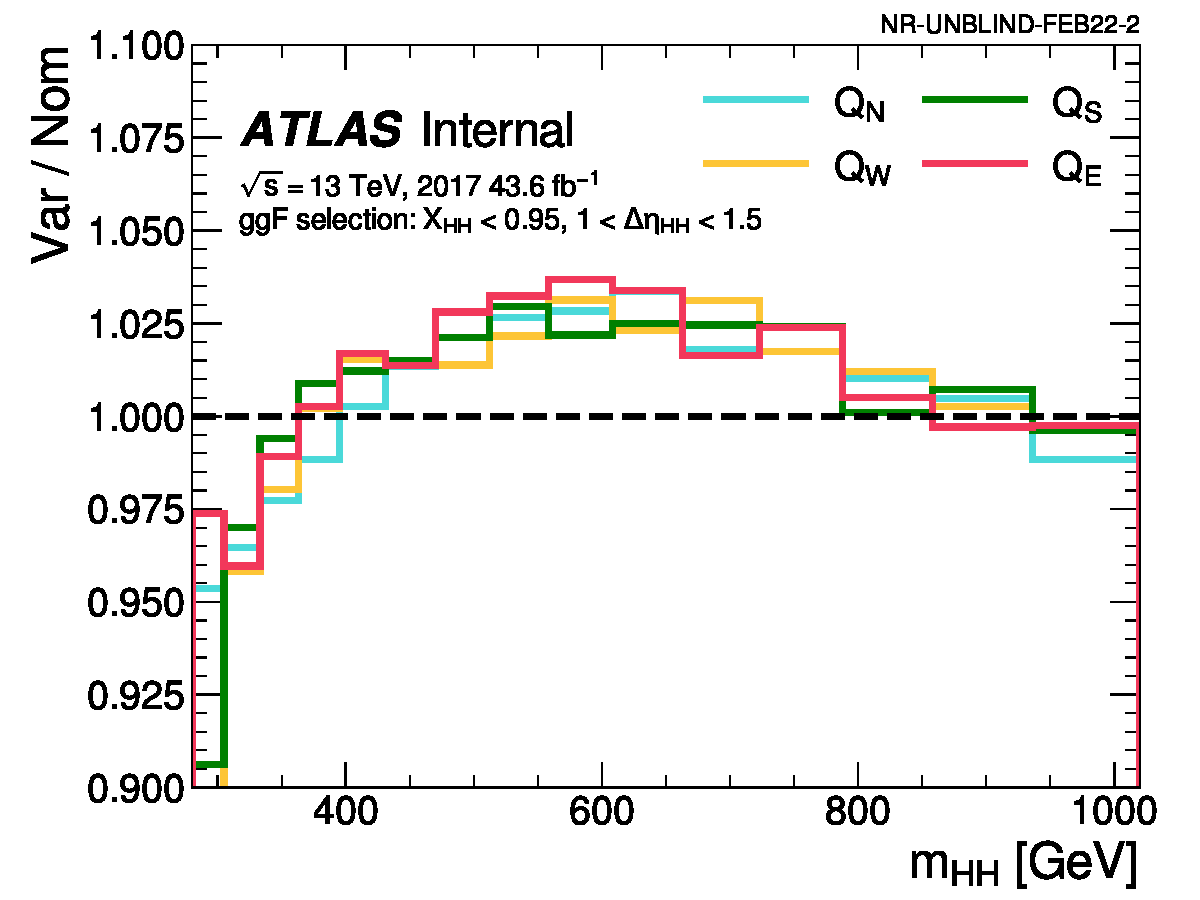
\includegraphics[width=0.3\textwidth]{\figpath/dEta_3_Xhh_1_17}
	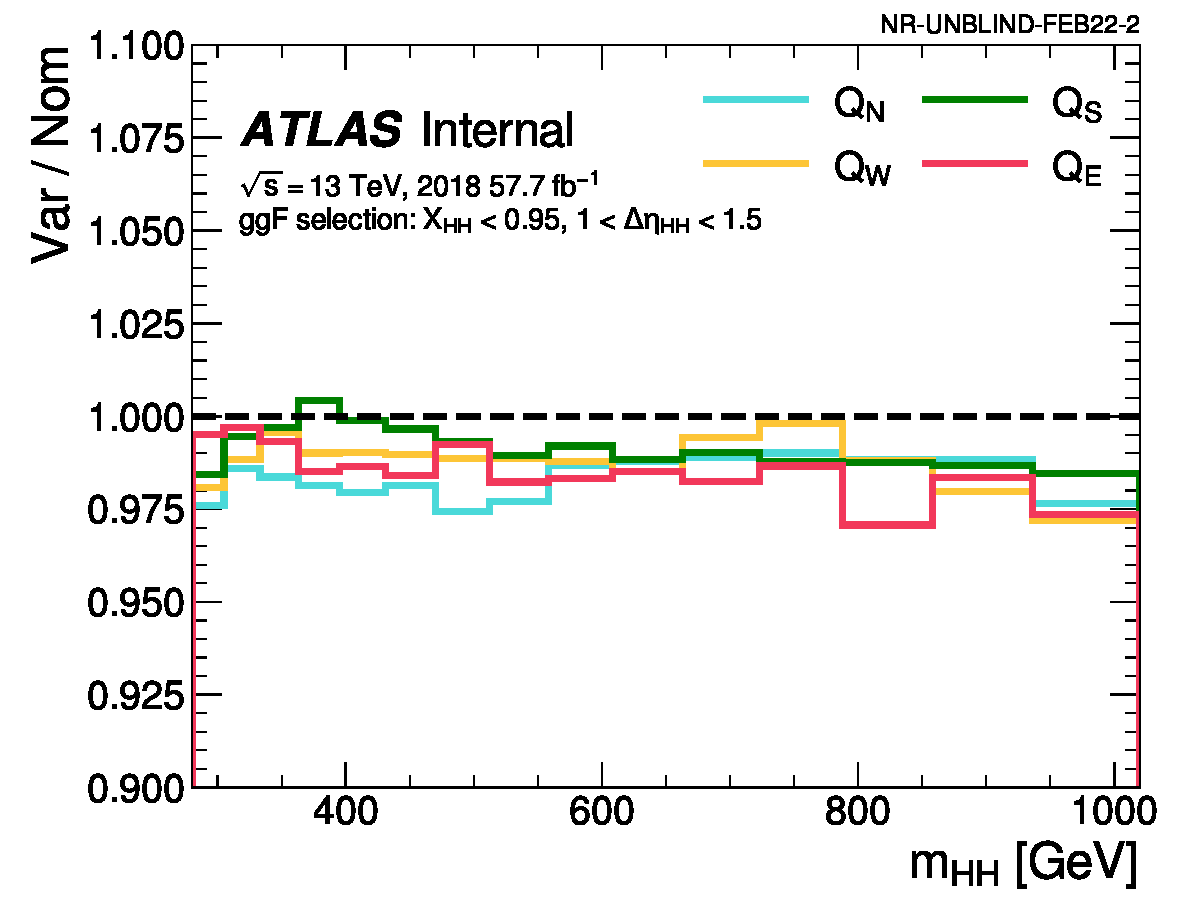
\includegraphics[width=0.3\textwidth]{\figpath/dEta_3_Xhh_1_18}
	\\
	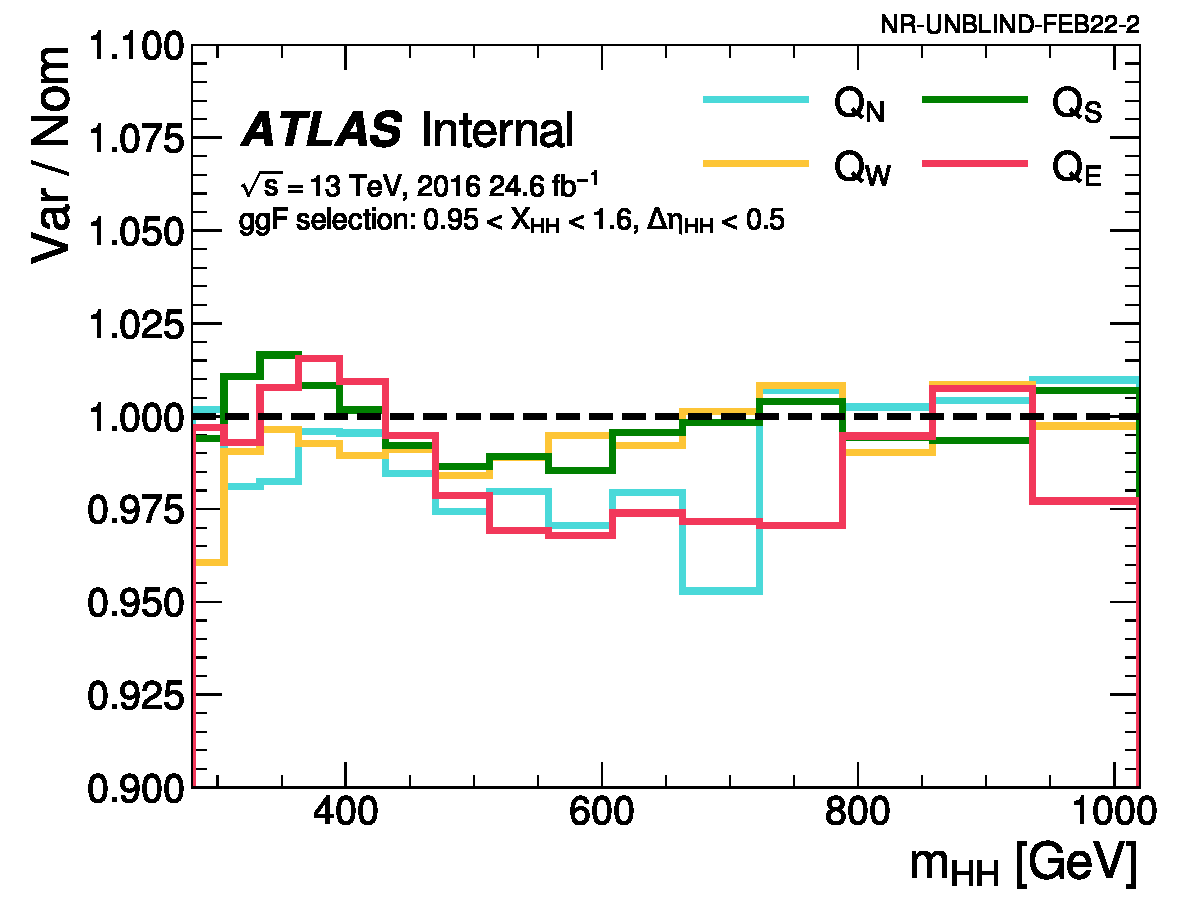
\includegraphics[width=0.3\textwidth]{\figpath/dEta_1_Xhh_2_16}
	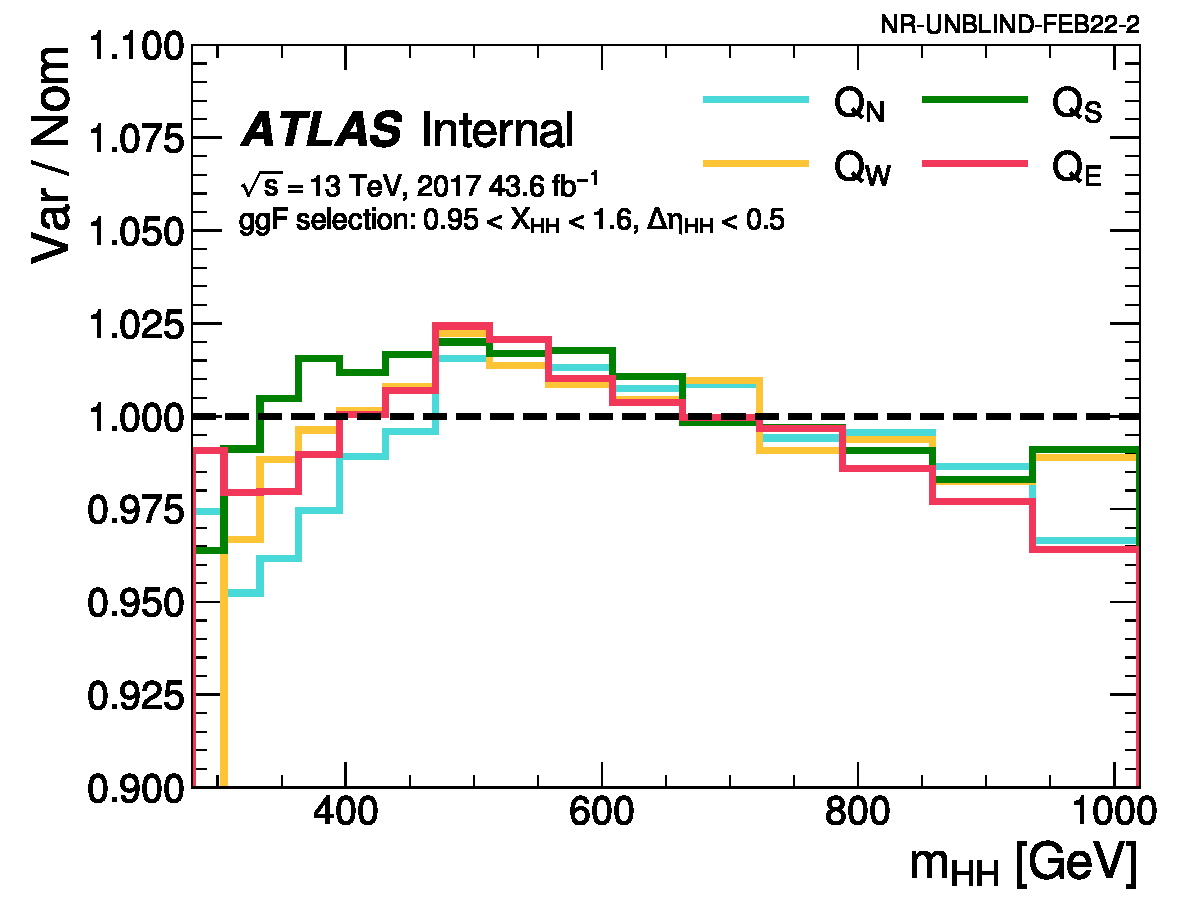
\includegraphics[width=0.3\textwidth]{\figpath/dEta_1_Xhh_2_17}
	\includegraphics[width=0.3\textwidth]{\figpath/dEta_1_Xhh_2_18}
	\\
	\includegraphics[width=0.3\textwidth]{\figpath/dEta_2_Xhh_2_16}
	\includegraphics[width=0.3\textwidth]{\figpath/dEta_2_Xhh_2_17}
	\includegraphics[width=0.3\textwidth]{\figpath/dEta_2_Xhh_2_18}
	\\
	\includegraphics[width=0.3\textwidth]{\figpath/dEta_3_Xhh_2_16}
	\includegraphics[width=0.3\textwidth]{\figpath/dEta_3_Xhh_2_17}
	\includegraphics[width=0.3\textwidth]{\figpath/dEta_3_Xhh_2_18}
	\caption{Impact of background shape nuisance parameter variation on \mhh in different kinematic categories for the ggF channel. Each column is a different years of the ggF channel templates while the rows show each category with the SR NP quadrants overlaid.}	 
	\label{fig:sr-np-impact-by-cat}
\end{figure}



The initial analysis unblinding occurred with a different nuisance parameter correlation scheme, where all parameters were treated as uncorrelated systematics.
This choice was made due to the lack of coherent variations in the different validation regions in the analysis, particularly the 3b1f region. Therefore, we believed giving flexibility for the fit to vary in different directions in different categories to be the best option. 
In addition, it was observed that the expected SR limits with the uncorrelated were more performant across different $\kappa_\lambda$ hypotheses. 
Results pertaining to this unblinding, which show clear indication and preference for the correlated scheme described above, can be seen in \App{\ref{app:unb-studies}}. This appendix also collects extensive studies on understanding these results.

\FloatBarrier




\FloatBarrier
\clearpage
\section{Background validation}
\label{sec:bkg-val-regns}

\begin{itemize}
\item Let's start off by re-showing the analysis graphic that I had before, but add \textbf{red text} for the inverted cuts!
\end{itemize}
